% CVPR 2022 Paper Template
% based on the CVPR template provided by Ming-Ming Cheng (https://github.com/MCG-NKU/CVPR_Template)
% modified and extended by Stefan Roth (stefan.roth@NOSPAMtu-darmstadt.de)

\documentclass[10pt,twocolumn,letterpaper]{article}

%%%%%%%%% PAPER TYPE  - PLEASE UPDATE FOR FINAL VERSION
\usepackage{cvpr}      % To produce the REVIEW version
%\usepackage{cvpr}              % To produce the CAMERA-READY version
%\usepackage[pagenumbers]{cvpr} % To force page numbers, e.g. for an arXiv version

% Include other packages here, before hyperref.
\usepackage{graphicx}
\usepackage{amsmath}
\usepackage{amssymb}
\usepackage{booktabs}
\usepackage{tabularx}
\usepackage{multirow}
\usepackage{makecell}
\usepackage{ulem}

% It is strongly recommended to use hyperref, especially for the review version.
% hyperref with option pagebackref eases the reviewers' job.
% Please disable hyperref *only* if you encounter grave issues, e.g. with the
% file validation for the camera-ready version.
%
% If you comment hyperref and then uncomment it, you should delete
% ReviewTempalte.aux before re-running LaTeX.
% (Or just hit 'q' on the first LaTeX run, let it finish, and you
%  should be clear).
\usepackage[pagebackref,breaklinks,colorlinks]{hyperref}


% Support for easy cross-referencing
\usepackage[capitalize]{cleveref}
\crefname{section}{Sec.}{Secs.}
\Crefname{section}{Section}{Sections}
\Crefname{table}{Table}{Tables}
\crefname{table}{Tab.}{Tabs.}


%%%%%%%%% PAPER ID  - PLEASE UPDATE
\def\cvprPaperID{11345} % *** Enter the CVPR Paper ID here
\def\confName{CVPR}
\def\confYear{2025}
\begin{document}

%%%%%%%%% TITLE - PLEASE UPDATE
\title{Hallo3: Highly Dynamic and Realistic Portrait Image Animation with Diffusion Transformer Networks}

\author{Jiahao Cui\textsuperscript{1},
        Hui Li\textsuperscript{1},
        Yun Zhan\textsuperscript{1},
        Hanlin Shang\textsuperscript{1},
        Kaihui Cheng\textsuperscript{1},
        Yuqi Ma\textsuperscript{1},
        Shan Mu\textsuperscript{1},
        Hang Zhou\textsuperscript{2},\\
        Jingdong Wang\textsuperscript{2},\;\;\;
        Siyu Zhu\textsuperscript{1,3} \\
\textsuperscript{1}Fudan University, \;\;\textsuperscript{2}Baidu Inc,
\;\;\textsuperscript{3}Shanghai Academy of AI for Science
 \\
% {\tt\small xxx@xxx}
% For a paper whose authors are all at the same institution,
% omit the following lines up until the closing ``}''.
% Additional authors and addresses can be added with ``\and'',
% just like the second author.
% To save space, use either the email address or home page, not both
}
\maketitle

%%%%%%%%% ABSTRACT
\begin{abstract}
Existing methodologies for animating portrait images face significant challenges, particularly in handling non-frontal perspectives, rendering dynamic objects around the portrait, and generating immersive, realistic backgrounds.
In this paper, we introduce the first application of a pretrained transformer-based video generative model that demonstrates strong generalization capabilities and generates highly dynamic, realistic videos for portrait animation, effectively addressing these challenges.
The adoption of a new video backbone model makes previous U-Net-based methods for identity maintenance, audio conditioning, and video extrapolation inapplicable. To address this limitation, we design an identity reference network consisting of a causal 3D VAE combined with a stacked series of transformer layers, ensuring consistent facial identity across video sequences.
Additionally, we investigate various speech audio conditioning and motion frame mechanisms to enable the generation of continuous video driven by speech audio. Our method is validated through experiments on benchmark and newly proposed wild datasets, demonstrating substantial improvements over prior methods in generating realistic portraits characterized by diverse orientations within dynamic and immersive scenes. Further visualizations and the source code are available at: \href{https://fudan-generative-vision.github.io/hallo3/#/}{https://fudan-generative-vision.github.io/hallo3}.

\end{abstract}

%%%%%%%%% BODY TEXT
\begin{figure*}
    \centering
    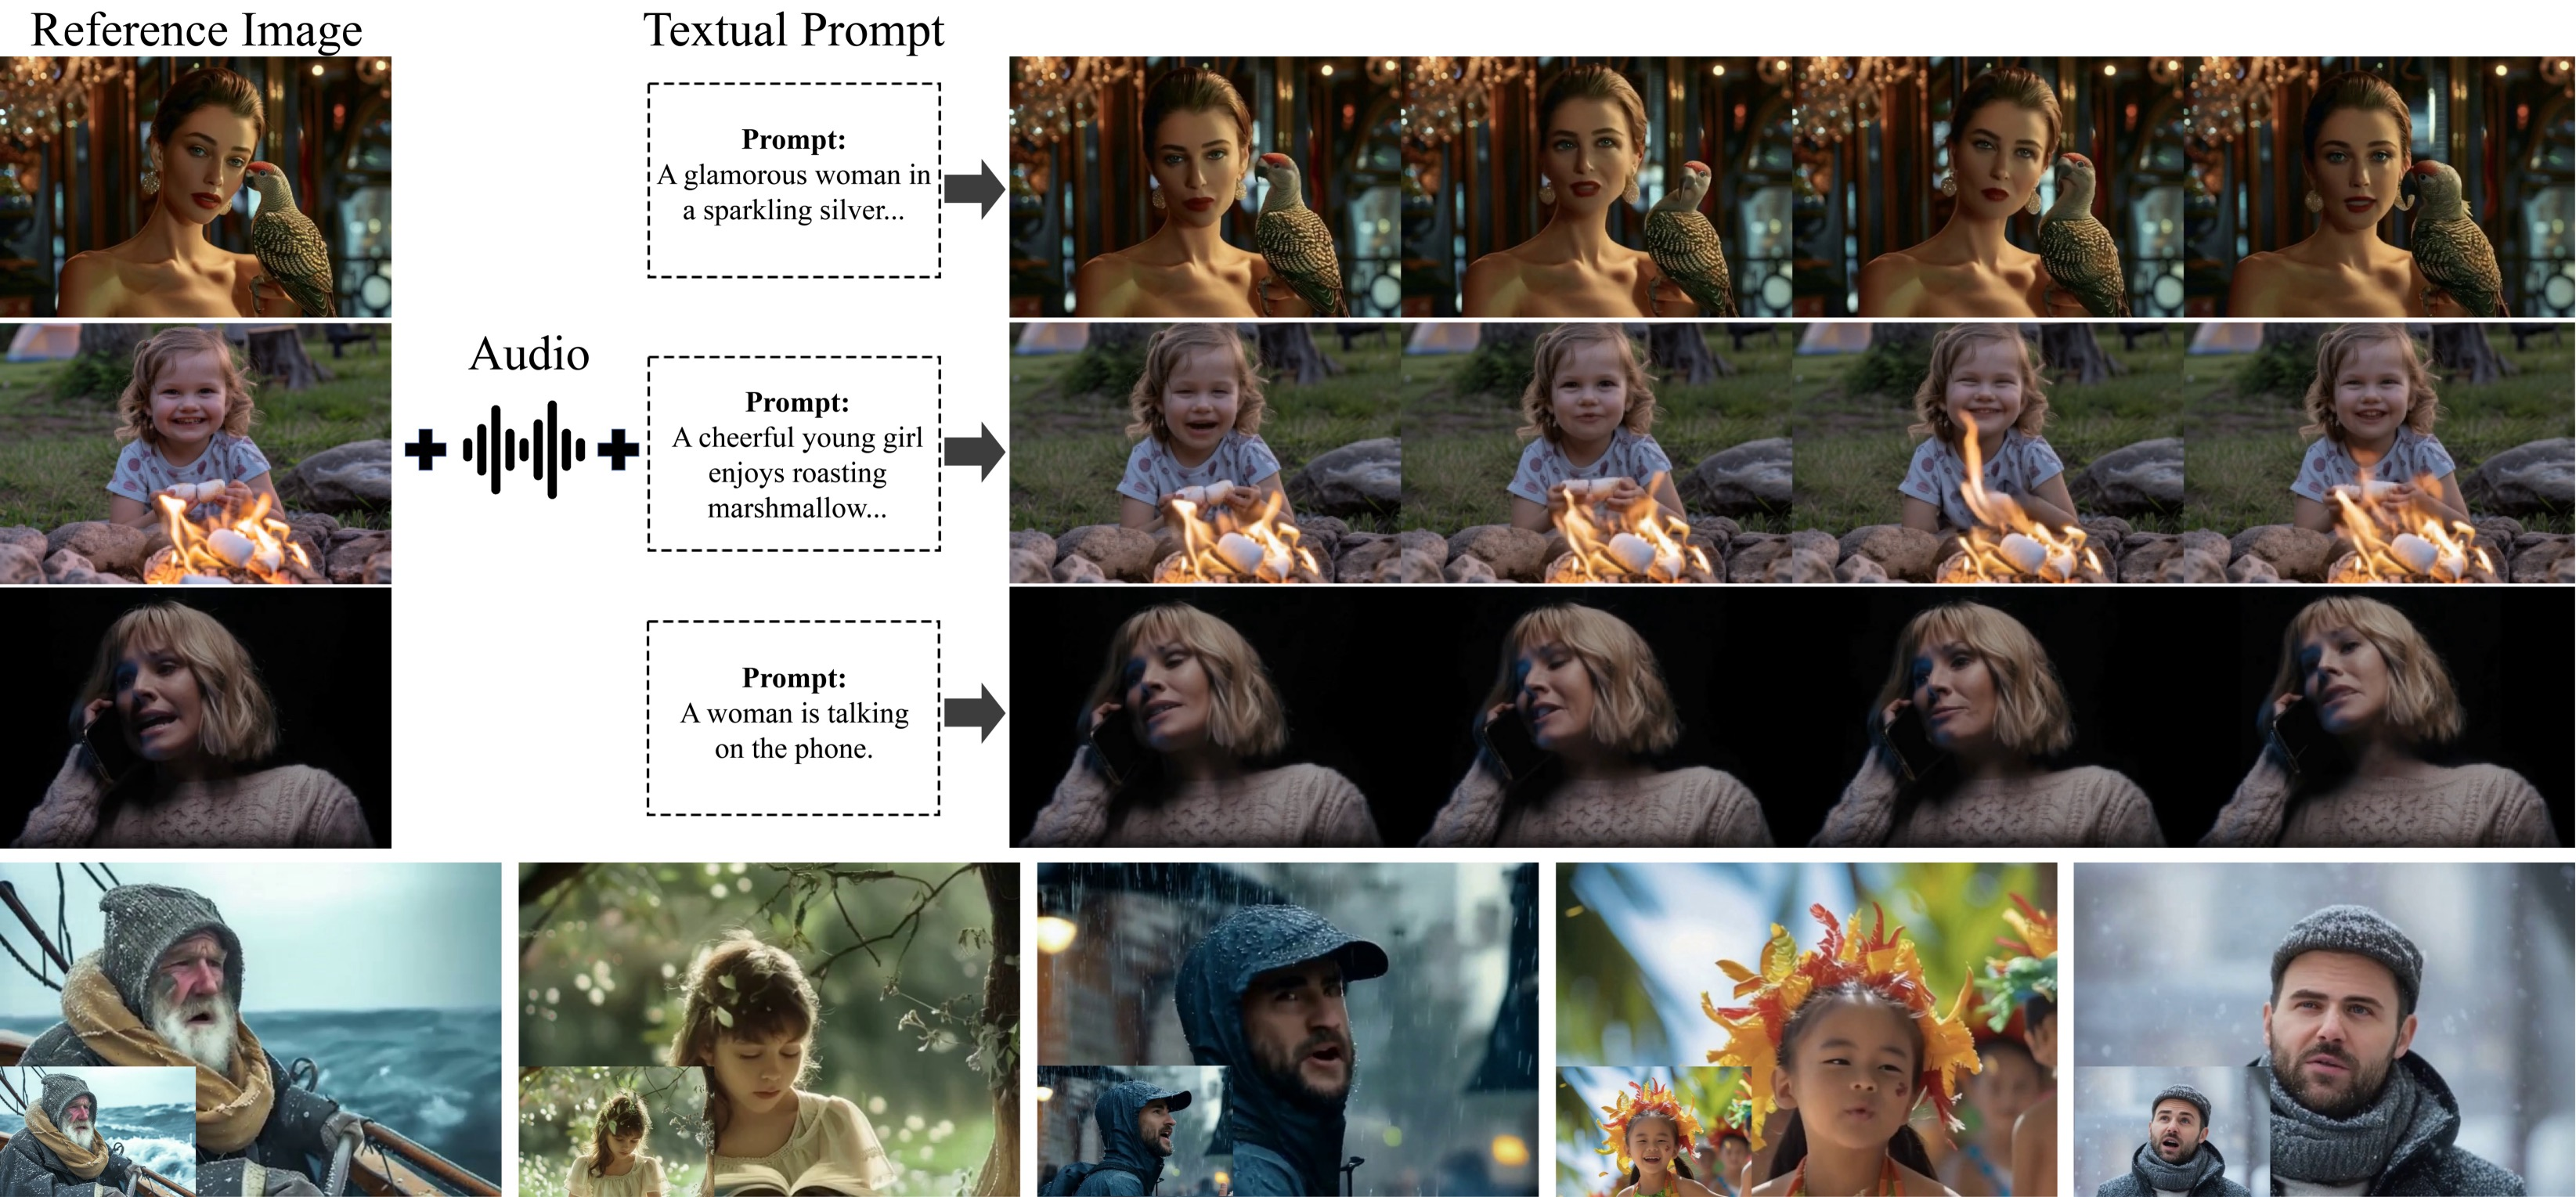
\includegraphics[width=1\linewidth]{figs/teaser.jpg}
    \caption{Demonstration of the proposed approach. Given a reference image, an audio sequence, and a textual prompt, the method generates animated portraits from frontal or different perspectives while preserving the portrait identity over extended durations. Additionally, it incorporates dynamic foreground and background elements, with temporal consistency and high visual fidelity. }
    \label{fig:enter-label}
    \vspace{-5mm}
\end{figure*}

\section{Introduction}
Portrait image animation refers to the process of generating realistic facial expressions, lip movements, and head poses based on portrait images. 
This technique leverages various motion signals, including audio, textual prompts, facial keypoints, and dense motion flow. 
As a cross-disciplinary research task within the realms of computer vision and computer graphics, this area has garnered increasing attention from both academic and industrial communities. 
Furthermore, portrait image animation has critical applications across several sectors, including film and animation production, game development, social media content creation, and online education and training.

In recent years, the field of portrait image animation has witnessed rapid advancements. 
Early methodologies predominantly employed facial landmarks—key points~\cite{siarohin2019first,zakharov2020fast,zhang2022sadtalker} on the face utilized for the localization and representation of critical regions such as the mouth, eyes, eyebrows, nose, and jawline. 
Additionally, these methods~\cite{gao2023high,ren2021pirenderer,zhang2023metaportrait,champ2024} incorporated 3D parametric models, notably the 3D Morphable Model (3DMM)~\cite{blanz2003face}, which captures variability in human faces through a statistical shape model integrated with a texture model. 
However, the application of explicit approaches grounded in intermediate facial representations is constrained by the accuracy of expression and head pose reconstruction, as well as the richness and precision of the resultant expressions.
Simultaneously, significant advancements in Generative Adversarial Networks (GANs) and diffusion models have notably benefited portrait image animation. 
These advancements~\cite{corona2024vlogger,liu2024anitalker,tian2024emo,wei2024aniportrait,xu2024vasa,zhang2024tora,champ2024} enhance the high-resolution and high-quality generation of realistic facial details, facilitate generalized character animation, and enable long-term identity preservation. 
Recent contributions to the field—including Live Portrait~\cite{guo2024liveportrait}, which leverages GAN technology for portrait animation with stitching and retargeting control, as well as various end-to-end methods such as VASA-1~\cite{xu2024vasa}, EMO~\cite{tian2024emo}, and Hallo~\cite{xu2024hallo,cui2024hallo2} employing diffusion models—exemplify these advancements.

Despite these improvements, existing methodologies encounter substantial limitations. 
First, many current facial animation techniques emphasize eye gaze, lip synchronization, and head posture while often depending on reference portrait images that present a frontal, centered view of the subject. 
This reliance presents challenges in handling profile, overhead, or low-angle perspectives for portrait animation. Secondly, accounting for significant accessories, such as holding a smartphone, microphone, or wearing closely fitted objects, presents challenges in generating realistic motion for the associated objects within video sequences.
Third, existing methods often assume static backgrounds, undermining their ability to generate authentic video effects in dynamic scenarios, such as those with campfires in the foreground or crowded street scenes in the background.

Recent advancements in diffusion transformer~(DiT)-based video generation models~\cite{yang2024cogvideox, polyak2024movie, bao2024vidu, liu2024sora} have addressed several challenges associated with traditional video generation techniques, including issues of realism, dynamic movement, and subject generalization. 
In this paper, we present the first application of a pretrained DiT-based video generative model to the task of portrait image animation.
The introduction of this new video backbone model renders previous U-Net-based methods for identity maintenance, audio conditioning, and video extrapolation impractical. 
We tackle these issues from three distinct perspectives.
(1)~\textbf{Identity preservation}: We employ a 3D VAE in conjunction with a stack of transformer layers as an identity reference network, enabling the embedding and injection of identity information into the denoising latent codes for self-attention. This facilitates accurate representation and long-term preservation of the facial subject's identity.
(2)~\textbf{Speech audio conditioning}: We achieve high alignment between speech audio—serving as motion control information—and facial expression dynamics during training, which allows for precise control during inference. We investigate the use of adaptive layer normalization and cross-attention strategies, effectively integrating audio embeddings through the latter.
(3)~\textbf{Video extrapolation}: Addressing the limitations of the DiT-based model in generating continuous videos, which is constrained to a maximum of several tens of frames, we propose a strategy for long-duration video extrapolation. 
This approach uses motion frames as conditional information, wherein the final frames of each generated video serve as inputs for subsequent clip generation.

We validate our approach using benchmark datasets, including HTDF and Celeb-V, demonstrating results comparable to previous methods that are constrained to limited datasets characterized by frontal, centered faces, static backgrounds, and defined expressions. 
Furthermore, our method successfully generates dynamic foregrounds and backgrounds, accommodating complex poses, such as profile views or interactions involving devices like smartphones and microphones, yielding realistic and smoothly animated motion, thereby addressing challenges that previous methodologies have struggled to resolve effectively. 
%
\section{Related Work}
%


\subsection{Classical Approaches} \label{appendix:related_work_classical}

Classical approaches in time series modeling include the Box-Jenkins method \citep{box1968some}, exponential smoothing  \citep{hyndman2008forecasting, winters1960forecasting}, autoregressive integrated moving average (ARIMA) \citep{box1970time}, and state-space models \citep{hamilton1994state}. In such approaches, the model is usually manually selected based analyzing time series features (e.g., seasonality and order of non-stationarity), where the selected model is then fitted for each individual time series. While classical approaches may be more interpretable than recent deep learning techniques, the domain expertise and manual labor needed to succesfully apply them renders them infeasible to the common setting of modeling thousands, or millions, of time series.

\subsection{Deep Learning Approaches} \label{appendix:related_work_deep}

% (Deep AR, LSTMs, RNNs)
\textbf{Recurrent models.}  Common deep learning architectures for modeling sequence data are the family of recurrent neural networks, which include GRUs~\citep{chung2014empirical}, LSTMs~\citep{hochreiter1997long}, and DeepAR \citep{salinas2020deepar}. However, due to the recurrent nature of RNNs, they are slow to train and may suffer from vanishing/exploding gradients, making them difficult to train \citep{pascanu2013difficulty}. \\

\textbf{Deep State Space models.} Recent work has investigated combining the expressive strengths of SSMs with the scalable strengths of deep neural networks \citep{rangapuram2018, gu2021efficiently}. \cite{rangapuram2018} propose to train a global RNN that transforms input covariates to sequence-spcific SSM parameters; however, one downside of this approach is that they inherit the drawbacks of RNNs. More recent approaches, such as LSSL \citep{gu2021combining}, S4 \citep{gu2021efficiently}, S4D \citep{gu2022parameterization}, and S5 \citep{smith2022simplified}, directly parameterize the layers of a neural network with multiple linear SSMs, and overcome common recurrent training drawbacks by leveraging the convolutional view of SSMs. While deep SSM models have been shown great promise in time series modeling, we show in our work -- which builds off deep SSMs -- that current deep SSM approaches are not able to capture autoregressive processes due to their continuous nature.  \\


\textbf{Neural differential equations as nonlinear state spaces.}
%
\citep{chen2018neural} parametrizes the vector field of continuous--time autonomous systems. These models, termed \textit{Neural Differential Equations} (NDEs) have seen extensive application to time series and sequences, first by \cite{rubanova2019latent} and then by \cite{kidger2020neural,morrill2021neural,massaroli2021differentiable} with the notable extension to \textit{Neural Controlled Differential Equations} (Neural CDEs). Neural CDEs can be considered the continuous--time, nonlinear version of state space models and RNNs \citep{kidger2022neural}. Rather than introducing nonlinearity between linear state space layers, Neural CDEs model nonlinear systems driven by a control input. 

The NDE framework has been further applied by \cite{poli2019graph} to model graph time series via \textit{Neural Graph Differential Equations}. In \cite{queiruga2020continuous}, a continuous-depth ResNet generalization based on ODEs is proposed, and in \cite{kim2021stiff} numerical techniques to enable learning of stiff dynamical systems with Neural ODEs are investigated. The idea of parameterizing the vector field of a differential equation with a neural network, popularized by NDEs, can be traced back to earlier works \citep{funahashi1993approximation, zhang2014comprehensive, weinan2017proposal}. \\



\textbf{Transformers.} 
While RNNs and its variants have shown some success at time series modeling, a major limitation is their applicability to long input sequences. Since RNNs are recurrent by nature, they require long traversal paths to access past inputs, which leads to vanishing/exploding gradients and as a result struggle with capturing long-range dependencies. 

To counteract the long-range dependency problem with RNNs, a recent line of work considers Transformers for time series modeling. The motivation is that due to the attention mechanism, a Transformer can directly model dependencies between any two points in the input sequence, independently of how far apart the points are. However, the high expressivity of the attention mechanism comes at the cost of the time and space complexity being quadratic in sequence length, making Transformers infeasible for very long sequences. As a result, many works consider specialized Transformer architectures with sparse attention mechanisms to bring down the quadratic complexity. For example, \cite{beltagy2020longformer} propose LogSparse self-attention, where a cell attends to a subset of past cells (as opposed to all cells), where closer cells are attended to more frequently, proportional to the log of their distance, which brings down complexity from $\mathcal{O}(\ell^2)$ to $\mathcal{O}(\ell(\log \ell)^2)$. \cite{zhou2021informer} propose ProbSparse self-attention, which achieves $\mathcal{O}(\ell \log \ell)$ time and memory complexity, where they propose a generative style decoder to speed inference. \cite{liu2022pyraformer} propose a pyramidal attention mechanism which shows linear time and space complexity with sequence length. Autoformer \citep{wu2021autoformer} suggests more specialization is needed in time series with a decomposition forecasting architecture, which extracts long-term stationary trend from the seasonal series and utilizes an auto-correlation mechanism, which discovers the period-based dependencies. \cite{zhou2022fedformer} believes previous attempts of Transformer-based architectures do not capture global statistical properties, and to do so requires an attention mechanism in the frequency domain. Confromer \citep{gulati2020conformer} stacks convolutional and self-attention modules into a shared layer to combine the strengths of local interactions from convolutional modules and global interactions from self-attention modules. Perceiver AR \citep{hawthorne2022general} builds on the Perceiver architecture, which reduces the computational complexity of transformers by performing self-attention in a latent space, and extends Perceiver's applicability to causal autoregressive generation.

While these works have shown exciting progress on time series forecasting, their proposed architectures are specialized to handle specific time series settings (e.g., long input sequences, or seasonal sequences), and are commonly trained to output a fixed target horizon length \citep{zhou2021informer}, \ie{} as \emph{direct multi-step forecasting} (DMS) \cite{https://doi.org/10.1111/j.1467-6419.2007.00518.x}. Thus, while effective at specific forecasting tasks, their setups are not obviously applicable to a broad range of time series settings (such as forecasting arbitrary horizon lengths, or generalizing to classification or regression tasks).
%

Moreover, \cite{zeng2022transformers} showed that simpler alternatives to Transformers, such as data normalization plus a single linear layer (NLinear), can outperform these specialized Transformer architectures when similarly trained to predict the entire fixed forecasting horizons. Their results suggest that neither the attention mechanism nor the proposed modifications of these time series Transformers may be best suited for time series modeling. Instead, the success of these prior works  may just be from learning to forecast the entire horizon with fully connected dependencies between prior time-step inputs and future time-step outputs, where a fully connected linear layer is sufficient. \\

\textbf{Other deep learning methods.} Other works also investigate pure deep learning architectures with no explicit temporal components, and show these models can also perform well on time series forecasting. \cite{oreshkin2019n} propose N-BEATS, a deep architecture based on backward and forward residual links. Even simpler, \cite{zeng2022transformers} investigate single linear layer models for time series forecasting. Both works show that simple architectures are capable of achieving high performance for time series forecasting. In particular, with just data normalization, the NLinear model in \cite{zeng2022transformers} obtained state-of-the-art performance on the popular Informer benchmark~\cite{zhou2021informer}. Given an input sequence of past lag terms and a target output sequence of future horizon terms, for every horizon output their model simply learns the fully connected dependencies between that output and every input lag sample. However, FCNs such as NLinear also carry inefficient downsides. Unlike Transformers and SSM-based models, the number of parameters for FCNs scales directly with input and output sequence length, \ie{} $\mathcal{O}(\ell h)$ for $\ell$ inputs and $h$ outputs. Meanwhile, \ourmethod{} shows that the SSM can improve the modeling quality of deep architectures, while maintaining constant parameter count regardless of input or output length. Especially when forecasting long horizons, we achieve higher forecasting accuracy with smaller models.

% \header{S4}\\
%\section{Preliminary}\label{sec:preliminary}
Large language models (LLMs), pretrained on vast corpora, have demonstrated superior capabilities in context understanding and logical reasoning. 
These models have achieved remarkable success across a wide range of tasks in various domains, including natural language processing~\cite{DBLP:journals/corr/abs-2307-06435, DBLP:journals/csur/MinRSVNSAHR24,xu2024large} 
and 
computer vision~\cite{DBLP:conf/nips/LiuLWL23a,DBLP:journals/pami/ZhangHJL24,DBLP:journals/corr/abs-2306-16410}.
Mainstream LLMs, such as GPT~\cite{bubeck2023sparks}, LLaMA~\cite{DBLP:journals/corr/abs-2302-13971}, and DeepSeek~\cite{DBLP:conf/acl/DaiDZXGCLZYWXLH24}, 
are primarily built on the transformer architecture~\cite{vaswani2017attention}. 
To explore the role of Key-Value (KV) cache management in accelerating LLM computations,
we first outline the core components of the transformer model and then introduce the mechanisms for managing the KV cache
to accelerate the LLMs.
Important notations in this survey are summarized in Tab.~\ref{tab:notation}.




\subsection{Transformer Architecture}\label{ssec:transformer}
Transformers~\cite{vaswani2017attention} have become the backbone of LLMs due to their ability to efficiently capture long-range dependencies sequential data, such as text.
This capability makes them particularly well-suited for tasks like machine translation, text generation, and image captioning.
The transformer architecture follows an encoder-decoder structure, where most LLMs utilize only the decoder component.
We first introduce the core components of the Transformer decoder and then describe the critical auto-regressive generation mechanism. 
Particularly, we do not describe certain components in transformer, such as normalization, as they do not impact the understanding of KV cache management.

\begin{table}[t]
    \centering
    \caption{Notation Summary}
    \label{tab:notation}
    \begin{tabular}{c|l}
        \toprule
        \textbf{Symbol} & \textbf{Definition} \\
        \midrule
        $X$ & Input sequence of tokens \\ \hline
        
        $\mathbf{X}$ & Dense representations of  $X$ \\ \hline

        $d_x$ & Dimensionality of the input embeddings. \\\hline

        
        $\mathbf{E}$ & Embedding matrix $\mathbf{E} \in \mathbb{R}^{d_{\text{vocab}} \times d_x}$. \\ \hline
        
        $PE(X)$ & Positional encoding \\ \hline
        
        $\mathbf{Q}_i, \mathbf{K}_i, \mathbf{V}_i$ & Query, Key, and Value matrices \\  \hline

         $d_k, d_v$ & Query/Key and Value dimension \\\hline

        $\mathbf{W}_{Q_i}, \mathbf{W}_{K_i}, \mathbf{W}_{V_i}$ & Weight matrices for computing $\mathbf{Q}_i, \mathbf{K}_i, \mathbf{V}_i$. \\\hline
        
        $\mathbf{Z}_i$ &  Self-attention Output  \\\hline
        
        $\mathbf{W}_O$ & Weight matrix \\\hline
        
        $\mathbf{W}_1, \mathbf{W}_2$ & Weight matrices \\ \hline
        
        $\mathbf{b}_1, \mathbf{b}_2$ & Bias vectors \\\hline
        
      %  $d_o$ & Dimensionality of the concatenated output of multiple attention heads. \\
       % $d_1, d_2$ & Dimensionality of intermediate and output layers in the Feed Forward Network (FFN). \\
       
        $t$ &  Sequence length index \\\hline
        
        $t_c$ & Number of tokens stored in the KV cache. \\ \hline
        
        $\mathbf{K}_i^t, \mathbf{V}_i^t$ & Key and Value at step $t$ \\ \hline        
        $\mathbf{\hat{K}}_i^{t-1}, \mathbf{\hat{V}}_i^{t-1}$ & Cached Key and Value \\\hline
        
        $h$ & Number of attention heads per layer \\\hline
        
        
        $L$ & Number of transformer layers \\\hline
        
      %  $\mathbf{h}_t$ & Hidden state of the LLM at decoding step $t$. \\
        
       % $\mathbf{W}_{\text{out}}, \mathbf{b}_{\text{out}}$ & Output projection matrix and bias vector for predicting the next token. \\
        
        $P(x_{t+1} | x_1, \cdots, x_t)$ & Conditional probability \\
       % $\text{Softmax}$ & Softmax function used to compute attention weights or output probabilities. \\
        \bottomrule
    \end{tabular}
\end{table}

\subsubsection{Transformer Decoder}\label{ssec:decoder}
As shown in Figure~\ref{fig:transformer}, a decoder-based transformer architecture is composed of multiple stacked Transformer blocks, each designed to process sequential data effectively. 
Typically, a Transformer block consists of two core components, i.e., a Multi-Head Self-Attention (MHSA) mechanism and a Feed Forward Network (FFN). 
These blocks are arranged sequentially, where the output of one block is passed as input to the next. This iterative design allows the model to refine its understanding of the input sequence progressively, making it highly effective for tasks such as text generation and language modeling.


\noindent \textbf{Positional Encoding.}
Before the input sequence is processed by the Transformer blocks, it undergoes a preprocessing phase. 
First, a tokenizer processes the input sentence $X$ by splitting it into discrete units, such as words or subwords. The resulting sequence can be represented as 
${X} = [x_1, x_2, \cdots, x_{|X|}]$.
These tokens are then mapped to dense vector representations using an embedding layer, i.e., $\mathbf{X} = \mathbf{I}_X  \mathbf{E}^{\top}$,
where $\mathbf{I}_{X} \in \{0,1\}^{n \times d_{\text{vocab}}}$ represents the one-hot vector of tokenized input $X$, $\mathbf{E} \in \mathbb{R}^{d_{\text{vocab}} \times d_x}$ is the embedding matrix, 
and $\mathbf{X}=[\mathbf{x}_1, \mathbf{x}_2, \cdots, \mathbf{x}_{|X|}]\in \mathbb{R}^{n \times d_{x}}$ is the resulting matrix of embedded token representations.
Since the Transformer architecture does not inherently account for the order of tokens in a sequence, \textbf{positional encodings} are added to the token embeddings $\mathbf{X}$ to incorporate positional information. This can be expressed as $\mathbf{X}=\mathbf{X}+ PE(X)$,
where $PE(X) \in \mathbb{R}^{n \times d_x}$ represents a function~\cite{zhao2023length,zheng2021rethinking,su2024roformer} (e.g., sine and cosine-based positional encoding) that generates positional embeddings for the input ${X}$.


\noindent \textbf{Transformer Block.}
Once the input features are prepared, they are passed through a series of stacked Transformer blocks. Each block begins with the Multi-Head Self-Attention (MHSA) mechanism, which captures both local and global dependencies. For each token, the self-attention mechanism computes a weighted sum over all other tokens in the sequence, where the weights are derived from the similarity between the tokens.
Particularly, since the operations within each transformer block are identical, we use a single transformer block as an example.
Specifically, given the input to a block, denoted as $\mathbf{X} \in \mathbb{R}^{|X| \times d}$, the MHSA mechanism computes the query vectors $\mathbf{Q}_i \in \mathbb{R}^{|X| \times d_k}$, key vectors $\mathbf{K}_i \in \mathbb{R}^{|X| \times d_k}$, and value vectors $\mathbf{V}_i \in \mathbb{R}^{|X| \times d_v}$. These vectors are obtained through learned linear transformations as follows:
\begin{align}\label{eq:qkv}
\mathbf{Q}_i = \mathbf{X}\mathbf{W}_{Q_i}, \quad
\mathbf{K}_i = \mathbf{X}\mathbf{W}_{K_i}, \quad
\mathbf{V}_i = \mathbf{X}\mathbf{W}_{V_i},
\end{align}
where $\mathbf{W}_{Q_i}\in \mathbb{R}^{d_x \times d_k}$, $\mathbf{W}_{K_i} \in \mathbb{R}^{d_x \times d_k}$
and $\mathbf{W}_{V_i} \in \mathbb{R}^{d_x \times d_v}$ are the learned weight parameters.
Then, the self-attention operation is applied to each triple $(\mathbf{Q}_i, \mathbf{K}_i, \mathbf{V}_i)$, and obtain  the output of the $i$-th attention head $\mathbf{Z}_i$ as follows:
\begin{equation}\label{eq:self_attention}
\mathbf{Z}_i = \text{Attention}(\mathbf{Q}_i, \mathbf{K}_i, \mathbf{V}_i) = \text{Softmax}\left(\frac{\mathbf{Q}_i \mathbf{K}_i^\top}{\sqrt{d_k}}\right) \mathbf{V}_i,
\end{equation}
where  $\sqrt{d_k}$  is a scaling factor to ensure the numerical stability. To capture diverse relationships, multiple attention with $h$ heads are applied to $\mathbf{X}$ in parallel, and their outputs are concatenated with one transformation as follows:
\begin{align}\label{eq:self_attention_concat}
\mathbf{Z}=\text{Concat}(\mathbf{Z}_1, \mathbf{Z}_2, \dots, \mathbf{Z}_h)\mathbf{W}_O,
\end{align}
where \text{Concat} is concatenation operation and $\mathbf{W}_O \in \mathbb{R}^{d_v \times d_o}$ is the trainable parameters.




Following the self-attention mechanism, 
the output is passed through a \textbf{Feed Forward Network (FFN)}. The FFN is a fully connected neural network that applies two linear transformations separated by a nonlinear activation function $\sigma(\cdot)$ (e.g, ReLU~\cite{agarap2018deep}) :
\begin{align}\label{eq:ffn}
    \text{FFN}(\mathbf{Z}) = \sigma(\mathbf{Z}\mathbf{W}_1 + \mathbf{b}_1)\mathbf{W}_2 + \mathbf{b}_2
\end{align}
where $\mathbf{W}_1 \in \mathbb{R}^{d_o \times d_1}$ and $\mathbf{W}_2 \in \mathbb{R}^{d_1 \times d_2}$ are  two  parameters.
Also, $\mathbf{b}_1 \in \mathbb{R}^{d_1}$ and $\mathbf{b}_2 \in \mathbb{R}^{d_2}$ are two bias vectors.

\subsubsection{Auto-regressive Generation Mechanism}\label{ssec:auto_regressive}
LLMs employ an autoregressive mechanism to generate text token by token, with each token conditioned on the previously generated ones. This iterative process ensures that the output sequence remains coherent and contextually appropriate.
Formally, given an input sequence of tokens $X = [x_1, x_2, \cdots, x_t]$, 
the model predicts the next token $x_{t+1}$ at each decoding step $t$ by modeling the conditional probability distribution as follows:
\begin{equation}
P(x_{t+1} | x_1, x_2, \cdots, x_t) = \text{Softmax}(\mathbf{h}_t \mathbf{W}_{\text{out}} + \mathbf{b}_{\text{out}}),
\end{equation}
where $\mathbf{h}_t \in \mathbb{R}^{d_h}$ represents the hidden state of the LLM regarding $X$ at step $t$, $\mathbf{W}_{\text{out}} \in \mathbb{R}^{d_h \times vocab}$ is the output projection matrix, and $\mathbf{b}_{\text{out}}$ is the bias vector. 
The softmax function converts the logits into a probability distribution over the vocabulary.
Then,
at each decoding step, the model generates the next token $x_{t+1}$ by sampling from the predicted probability distribution:
\begin{equation}
x_{t+1} \sim P(x_{t+1} | x_1, x_2, \cdots, x_t).
\end{equation}
The generated token $x_{t+1}$ is then appended to the sequence $X=[x_1,\cdots,x_t,x_{t+1}]$, and the process continues until a special end-of-sequence (EOS) token is generated or a predefined maximum length is reached.



 \begin{figure}[t]
    \centering
    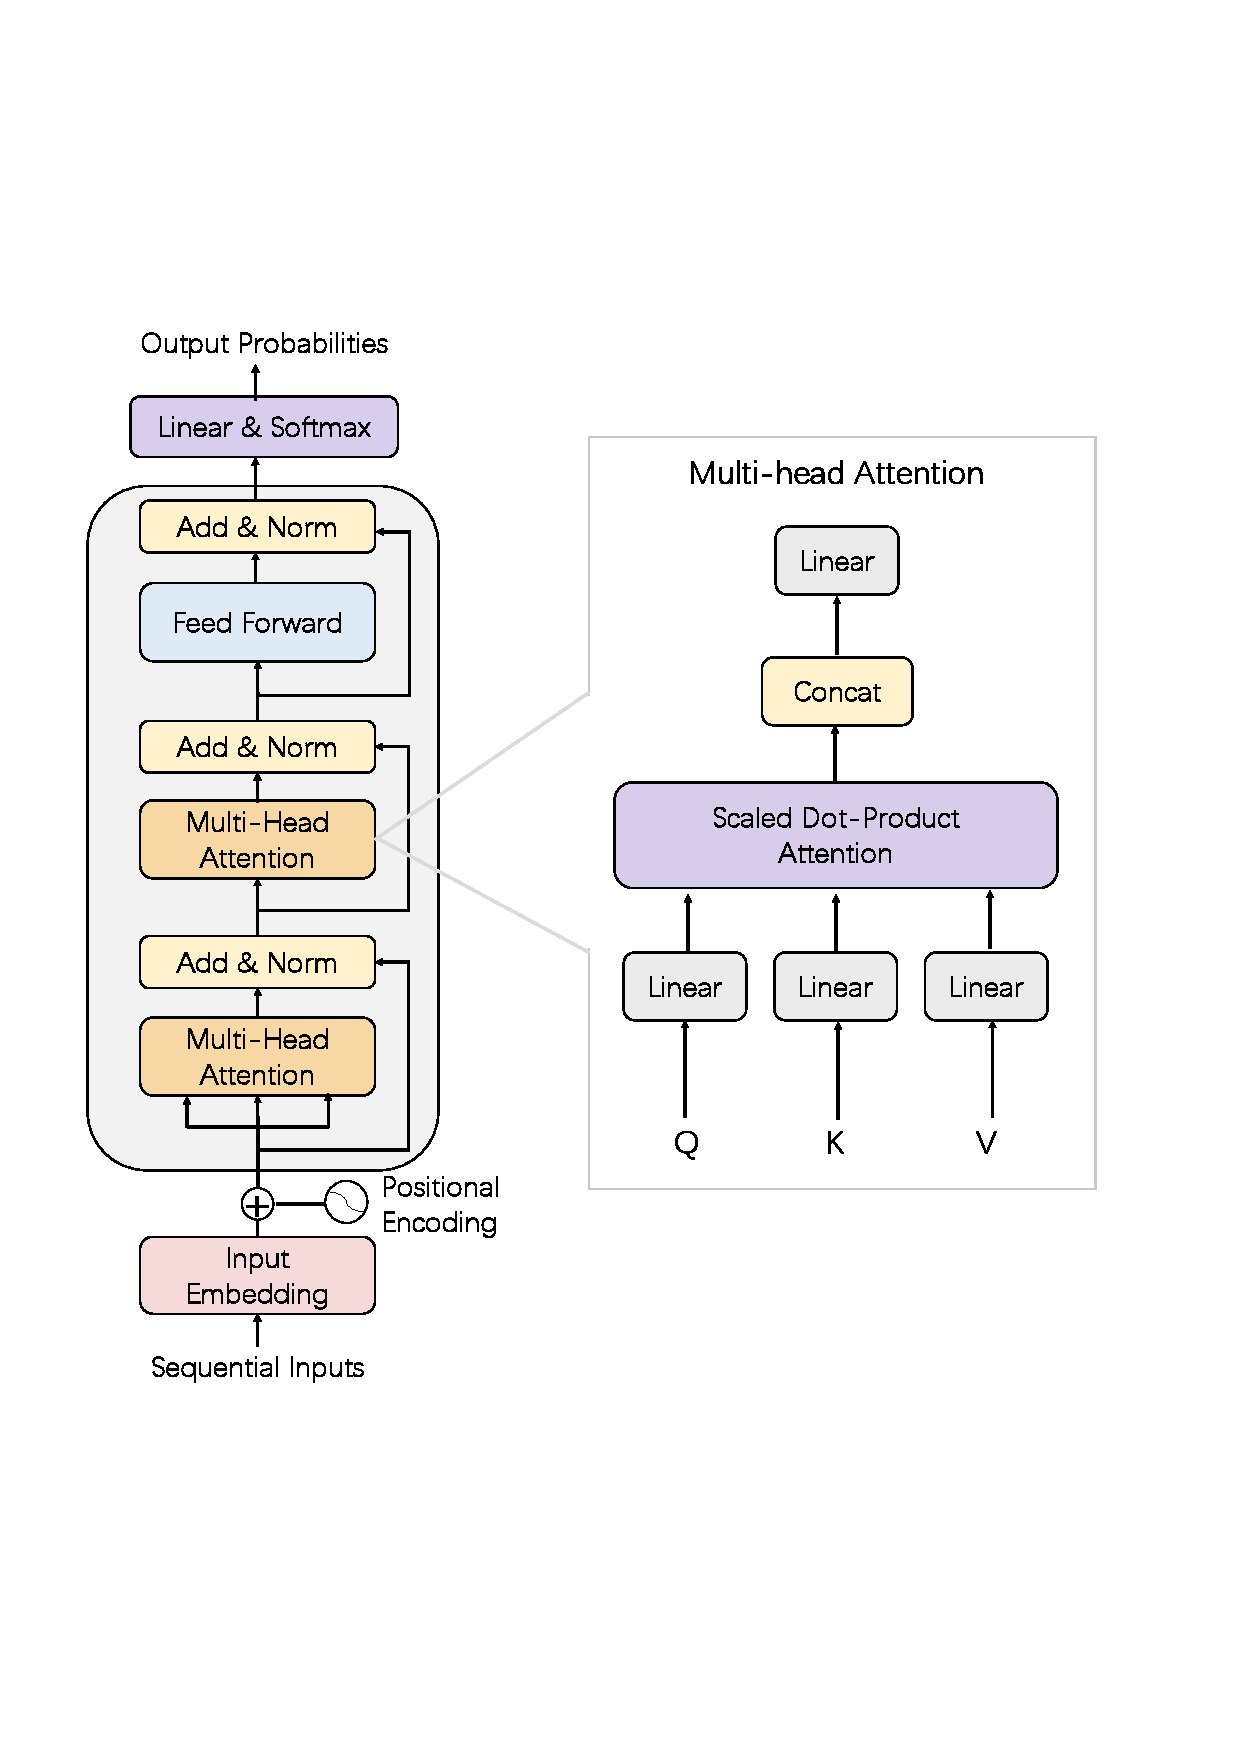
\includegraphics[width=0.88\linewidth]{figures/transfomer.pdf}
    \caption{The decoder-only Transformer for LLMs.}
    \label{fig:transformer}
\end{figure}


 


 

\subsection{Key-Value Cache in Transformer Models}\label{ssec:kv_cache}
Auto-regressive generation is a powerful mechanism that enables LLMs to produce high-quality, contextually coherent text. 
However, it presents computational challenges for long sequences, as the Keys and Values need to be recomputed for each token during the generation process. The KV cache optimization addresses this issue by storing the previously computed Keys and Values and reusing them for subsequent token generation, thereby reducing redundant computations and improving inference efficiency.


\subsubsection{Auto-regressive Generation with KV Cache}
Here, we describe how caching KV pairs of tokens accelerates LLM inference. Specifically, at each decoding step \( t \), the model performs self-attention over the entire sequence \( X = [x_1, \cdots, x_{t-1}, x_t] \) to generate the next token \( x_{t+1} \). This process requires the computation of Keys and Values matrices for all previously processed tokens in \( X = [x_1, \cdots, x_t] \).
Notably, when generating the token \( x_t \), the LLM has already computed the Keys and Values for the tokens in \( X[1:t-1] = [x_1, \cdots, x_{t-1}] \). The KV cache optimizes this process by storing the previously computed Keys and Values  matrices for \( X[1:t-1] \) and reusing them, thereby only requiring the computation of Keys and Values for the new token \( x_t \). This significantly improves efficiency by eliminating redundant computations.

Formally, at decoding step $t$, the new token embedding $\mathbf{x}_t$ is used to compute the query vector $\mathbf{q}^t_i$, key vector $\mathbf{k}^t_i$, and value vector $\mathbf{v}^t_i$ as follows:
\begin{align}
\mathbf{q}_i^t &= \mathbf{x}_t \mathbf{W}_{Q_i}, \quad
\mathbf{k}_i^t  = \mathbf{x}_t \mathbf{W}_{K_i}, \quad
\mathbf{v}_i^t  = \mathbf{x}_t \mathbf{W}_{V_i},
\end{align}
The newly computed $\mathbf{k}_i^t $ and $\mathbf{v}_i^t $ are then appended to the cached key and value matrices from previous steps:
\begin{align}
\mathbf{K}_i^{t} &= \text{Concat}(\mathbf{\hat{K}}_i^{t-1}, \mathbf{k}_i^t ), \ 
\mathbf{V}_i^{t} = \text{Concat}(\mathbf{\hat{V}}^{t-1}_i, \mathbf{V}_i^t ),
\end{align}
where $\mathbf{\hat{K}}_i^{t-1} \in \mathbb{R}^{t-1 \times d_k}$ and $\mathbf{\hat{V}}_i^{t-1} \in \mathbb{R}^{t-1 \times d_v}$ represent the cached key and value matrices of tokens in $X[1:t-1]$. 
These cached matrices are then used in the scaled dot-product attention computation for token $x_t$.
%which avoids re-computing attention for previously processed tokens. 
The attention output $\mathbf{z}^t_i$ for the token $x_t$ at step $t$ is calculated as:
\begin{align}
\mathbf{z}^t_i = \text{Softmax}\left(\frac{\mathbf{q}_i^t {\mathbf{K}_i^t}^\top}{\sqrt{d_k}}\right) \mathbf{V}_i^t,
\end{align}
\noindent Then, a similar KV reuse process can be applied to different attention heads in each layer of the LLM.


 
 

\subsubsection{Time and Space Complexity Analysis}\label{sssec:time_space}
Given a transformer-based $L$-layer LLM with $h$ attention heads per layer and an input sequence of length $X = [x_1, \cdots, x_t]$, we analyze the time saved and the space required to store cached KV pairs. For simplicity, we assume the Keys and Values of $t_c$ tokens are stored for all heads across all LLM layers.

\noindent \underline{\textbf{Saved Time.}} 
    For each token,
    the saved computation time comes from avoiding the repeated computation of Keys and Values in Equation~\eqref{eq:qkv}, self-attention result in Equation~\eqref{eq:self_attention}, 
    and linear transformation  in  Equation~\eqref{eq:self_attention_concat}.
     We omit the time analyze on operations in transformer that do not affect  the understanding of KV cache acceleration, such as layer norm and position encoding.

    %and non-linear transformation  in  Equation~\eqref{eq:self_attention_concat} and~\eqref{eq:ffn}.
\begin{itemize}[leftmargin=10pt]
    \item \textbf{QKV Computation.} 
    The time of computing Queries, Keys and Values for each token in Equation~\eqref{eq:qkv} is $\triangle_1 = O(2d_xd_k + d_xd_v)$.
  
    \item  \textbf{Self-attention Result.} 
    Additionally, computing each attention result $\mathbf{z}_i$ in Equation~\eqref{eq:self_attention} takes $O(t(d_k + d_v))$.
    %where $t$ is the sequence length. 

   \item \textbf{Linear Transformation.}
    To merge the $h$ attention results in  Equation~\eqref{eq:self_attention_concat} 
    %and compute the forward result in Equation~\eqref{eq:ffn}, 
    the time is $\triangle_2 = O(hd_v+d_vd_o)$. 

\end{itemize}
Therefore, for $t_c$ cached tokens across $h$ attention heads and $L$ layers, the total saved computation time is:
\begin{align}
    %O\left(L\cdot h \cdot t_c \cdot t \cdot (d_k+d_v)+ L\cdot h \cdot t_c\cdot \triangle_1 \right)
    O\left(L\cdot h \cdot t_c \cdot t \cdot (d_k+d_v)+ L\cdot h \cdot t_c\left(\triangle_1 + \triangle_2\right)\right)
\end{align}
\noindent Thus, the saved time is directly proportional to the number of cached tokens $t_c$, 
significantly accelerating model computation, especially for longer sequences (when $t$ is large).



\noindent \underline{\textbf{Extra Space.}}
Compared to computation without caching, additional space is required to store the cached KV pairs for $t_c$ tokens across $h$ attention heads and $L$ layers. Assuming each Key and Value is stored in Float16 precision, the total extra space needed can be expressed as:
\begin{align}
    O(L\cdot h \cdot t_c \cdot 2 \cdot sizeof(Float16))    
\end{align}
\noindent 
Thus, for the same LLM model, the extra space required to store the KV pairs primarily depends on the number of cached tokens and the precision of the cached Keys and Values. 
To address this, existing approaches explore various techniques to reduce the extra space consumption, such as caching only the most important Keys and Values or applying quantization techniques to lower the bit precision of the stored Keys and Values.






 


\subsection{Challenges in KV Cache Management}\label{ssec:kv_cache_challenge}
As analyzed in Sec.~\ref{sssec:time_space}, 
reusing cached KV pairs enables the LLM to avoid recomputing past tokens, resulting in significant speedups during inference. However, as sequence lengths grow, the size of the KV cache increases proportionally, placing significant pressure on memory. Consequently, it becomes challenging to manage this cache effectively to accelerate LLM computation without excessive space usage.

\begin{itemize}[leftmargin=10pt]
    \item \textbf{Cache Eviction Policies:} 
    Determining which items to evict when the cache reaches its capacity is a complex problem. Popular policies~\cite{podlipnig2003survey} like Least Recently Used (LRU) or Least Frequently Used (LFU) do not align with LLMs  patterns, leading to suboptimal performance.

    \item \textbf{Memory Management:} 
    The memory required for the KV cache grows linearly with both the sequence length and the number of layers, which can quickly exceed the hardware memory limits, especially for long sequences. Consequently, managing the collaboration between different types of storage hardware (e.g., GPU, CPU, or external memory) becomes a significant challenge.




    
    \item \textbf{Latency Bottlenecks:} Accessing and updating the cache at each decoding step can introduce latency, particularly for hardware with limited memory bandwidth.

    \item \textbf{Compression Trade-offs:} Compressing the KV cache can reduce memory usage but may degrade model performance if key information is lost.

    \item \textbf{Dynamic Workloads:} Handling dynamic and unpredictable workloads, where access patterns and data requirements frequently change, requires adaptive caching strategies that can respond in real time.


    \item \textbf{Distributed Coordination:} In distributed KV caches, maintaining coordination across multiple nodes to ensure consistency, fault tolerance, and efficient resource usage adds significant complexity.

\end{itemize}
% \begin{figure*}[!t]
%     \centering
%     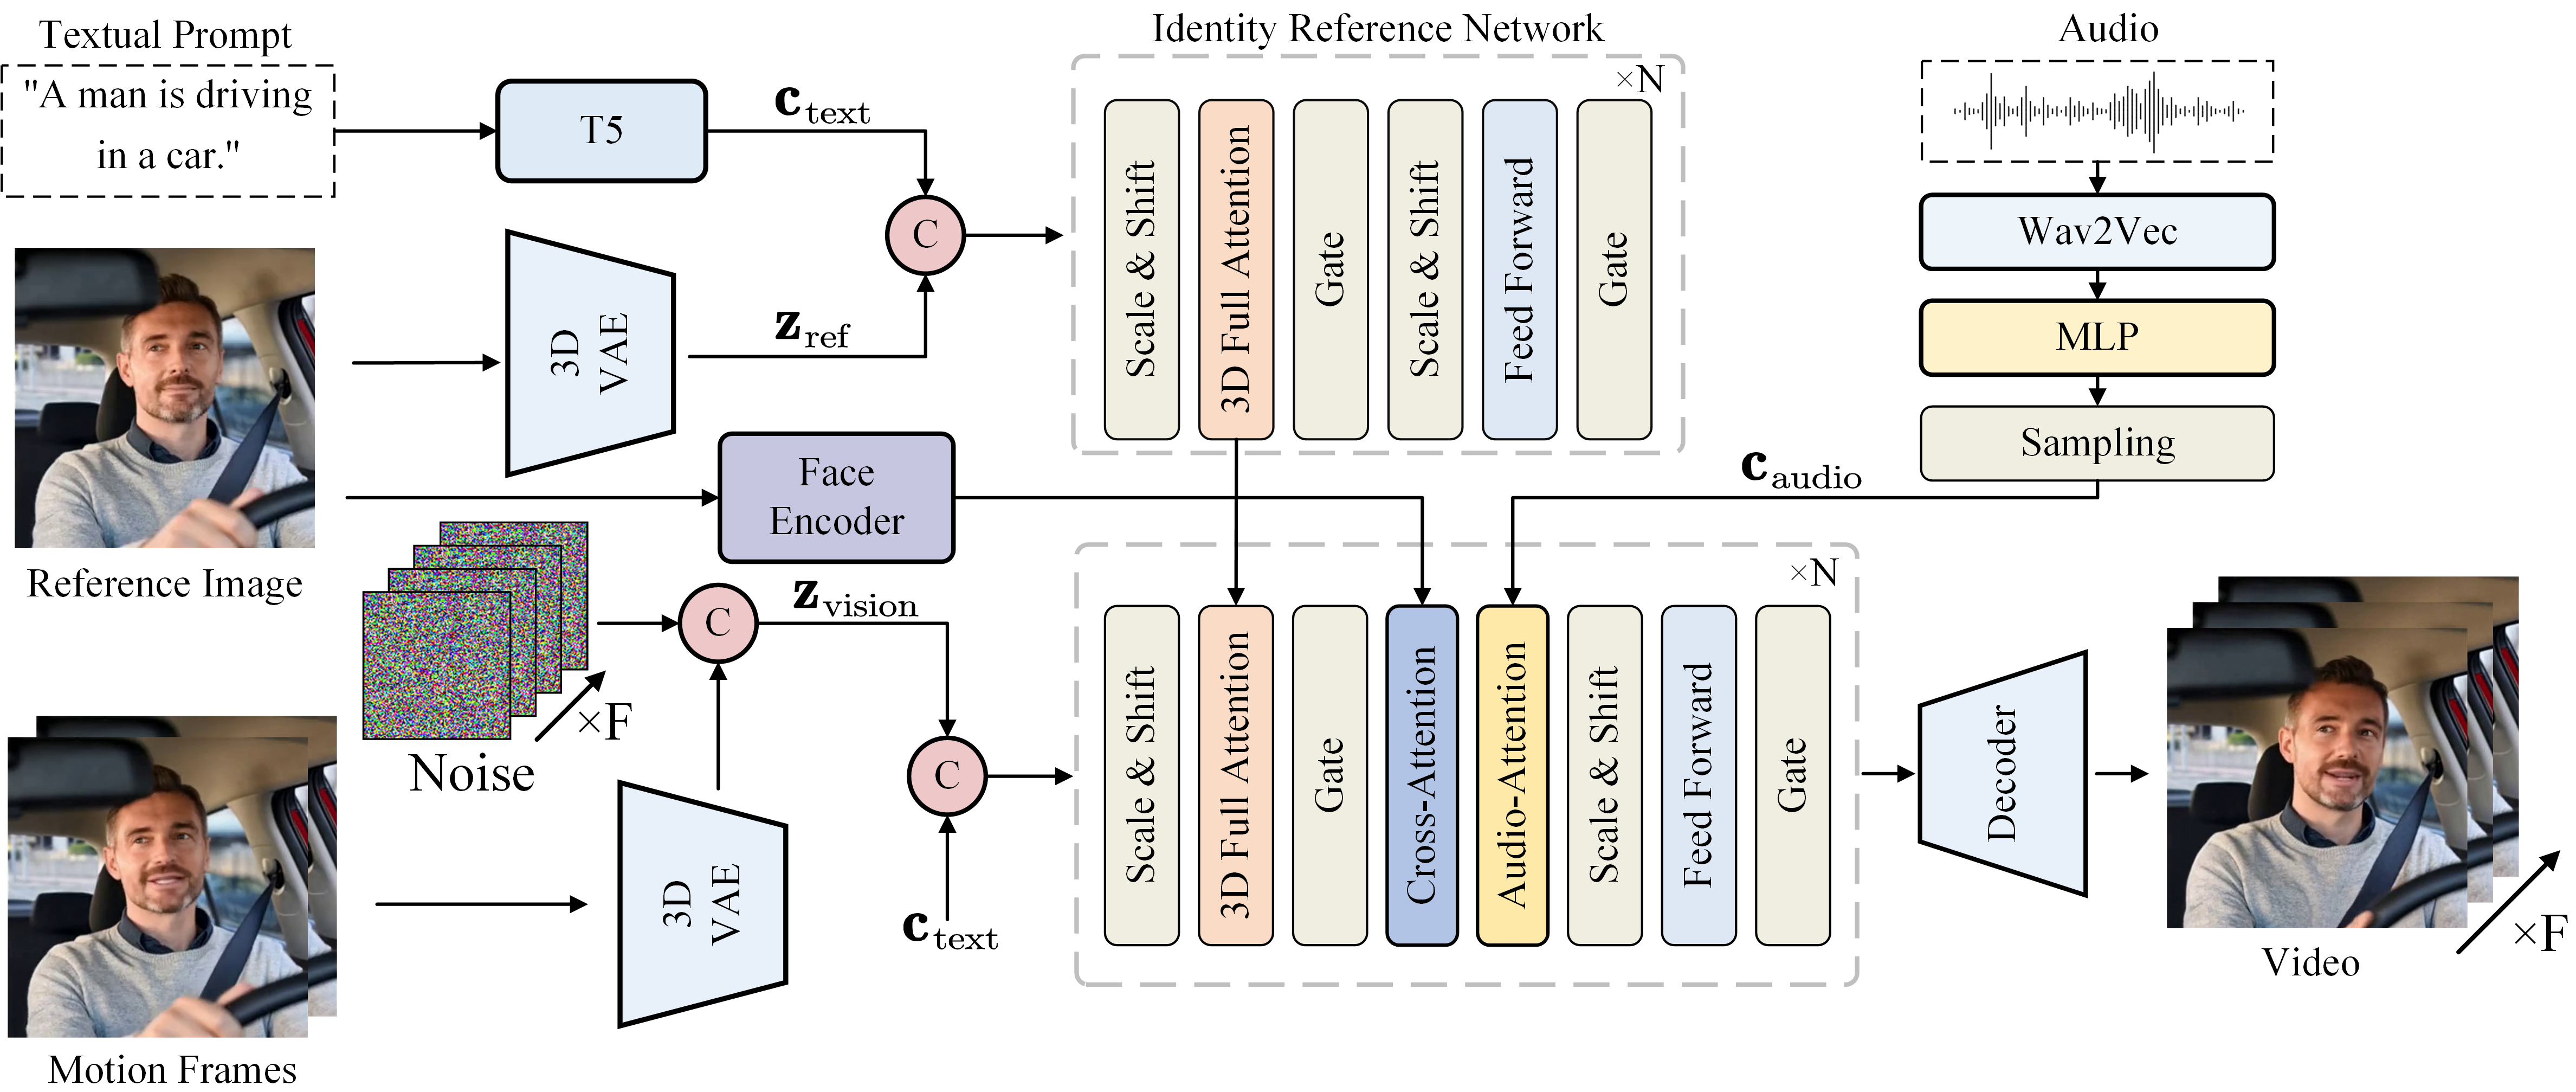
\includegraphics[width=1\linewidth]{figs/Pipeline.png}
%     \caption{The overview of the proposed method. Specifically, the method takes reference images, an audio sequence, and textual prompts as inputs to generate a video output with temporal consistency and high visual fidelity. We leverage the casual 3D VAE, T5, and Wav2Vec models to process the visual, textual, and audio features, respectively. The Identity Reference Network extracts identity features from the input reference images and textual prompts, enabling controllable animation while preserving the subject's appearance. The audio encoder generates motion information for lip synchronization, while the face encoder extracts facial features to maintain consistency in facial expressions. The 3D Full Attention and Audio-Attention Modules combine identity and motion data within a denoising network, producing high-fidelity, temporally consistent, and controllable animated videos.}
%     \label{fig:architecture}
%     \vspace{-4 mm}
% \end{figure*}


\begin{figure*}[t!]
    \centering

    % 左侧大图
    \begin{minipage}[b]{0.65\textwidth} % 左侧宽度占40%
        \centering
        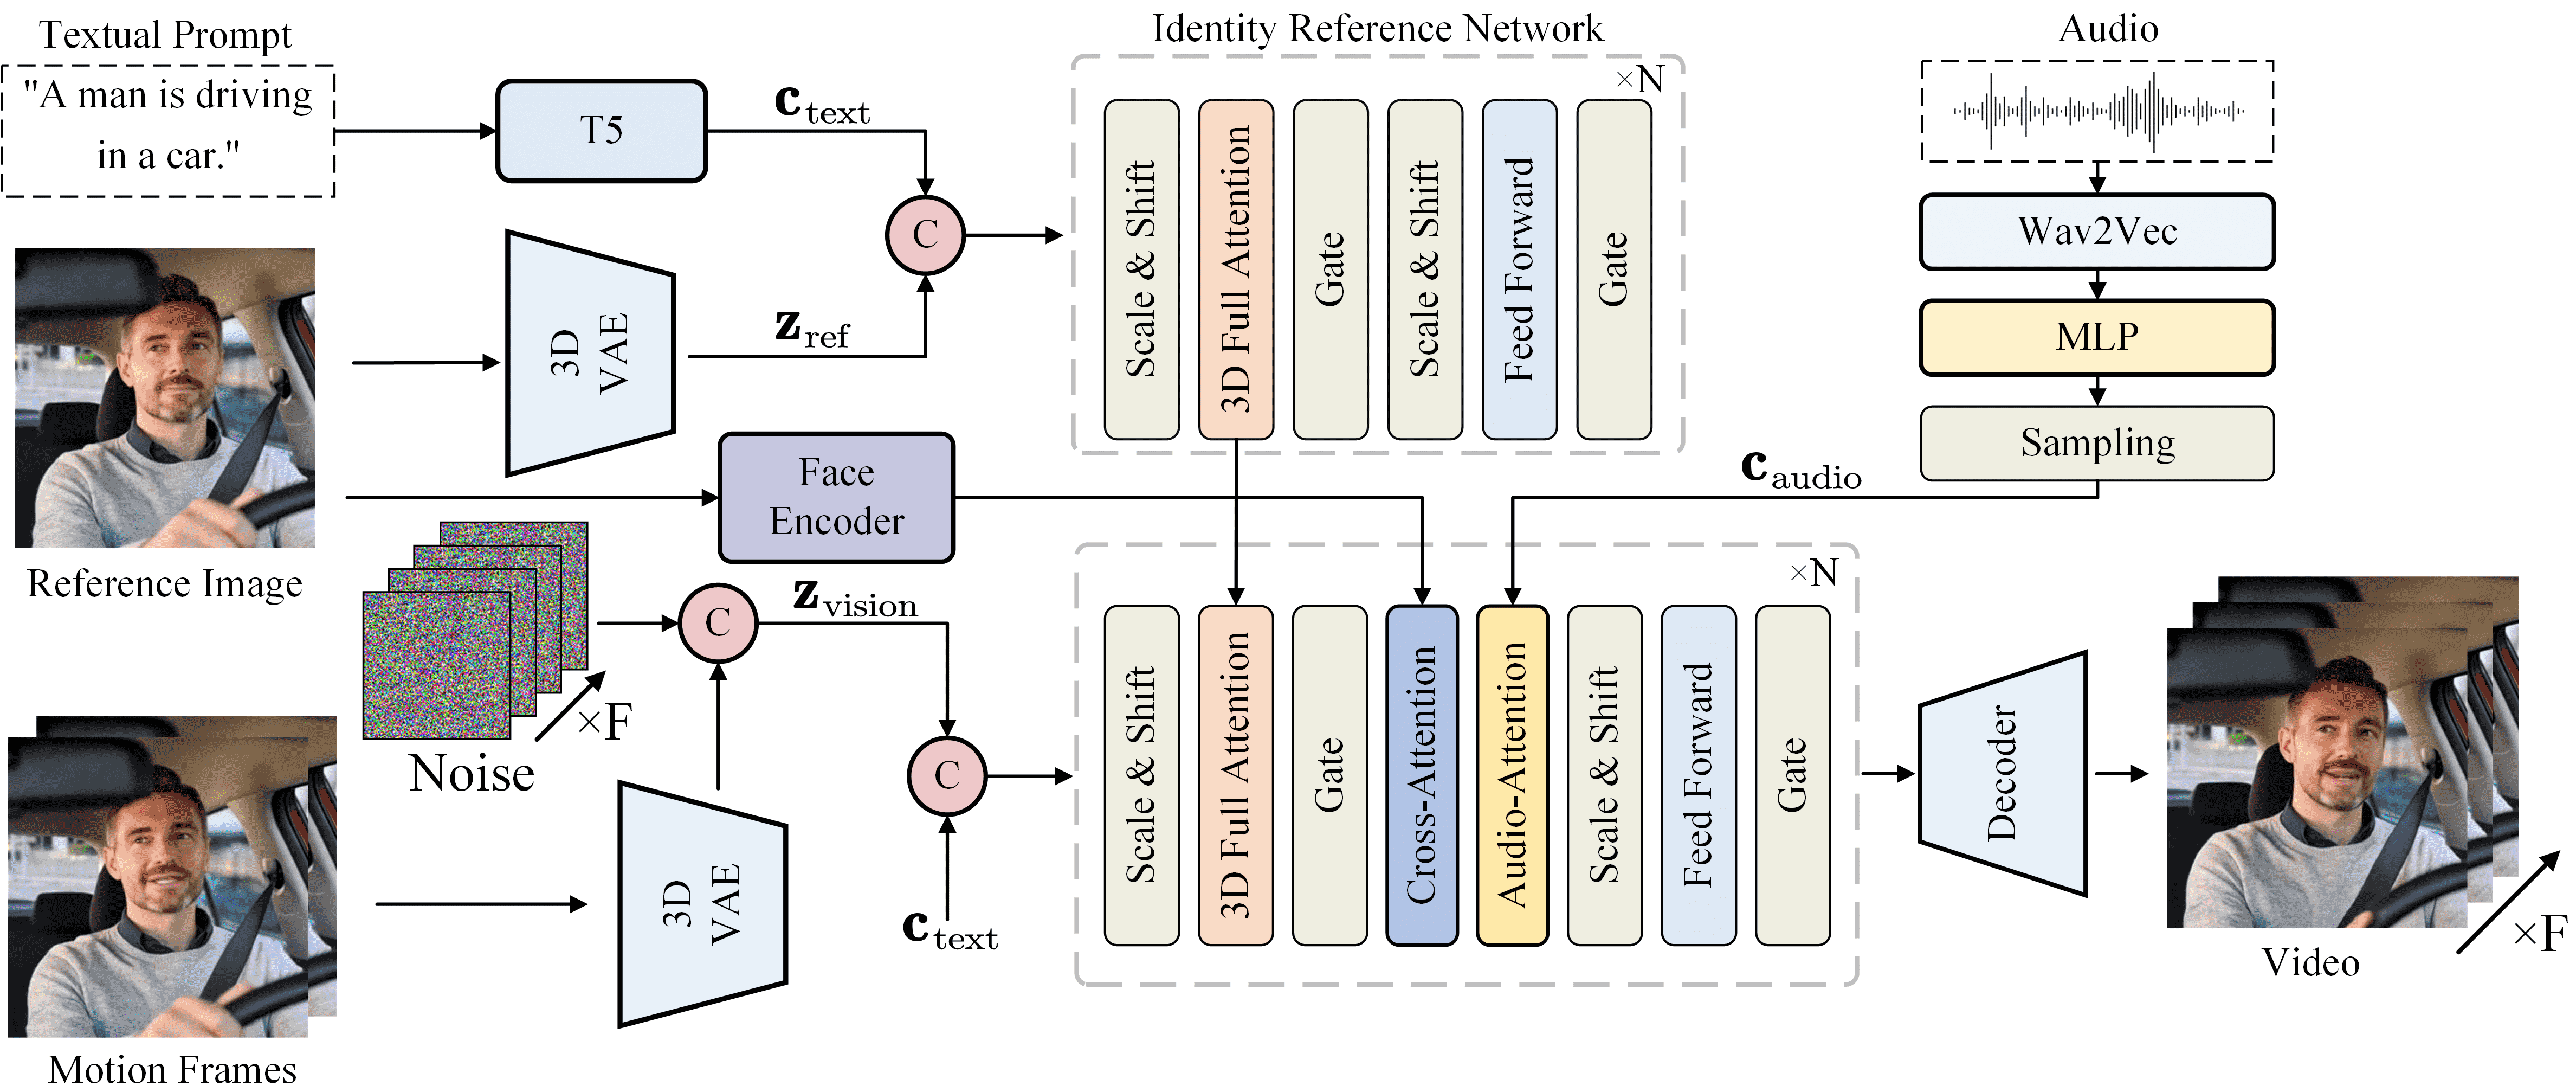
\includegraphics[width=\linewidth]{figs/Pipeline_comp.png} % 替换为你的图片路径
        \caption{The overview of the proposed method. Specifically, the method takes a reference image, an audio sequence, and a textual prompt as inputs to generate a video output with temporal consistency and high visual fidelity. We leverage the casual 3D VAE, T5, and Wav2Vec models to process the visual, textual, and audio features, respectively. The Identity Reference Network extracts identity features from the input reference image and textual prompt, enabling controllable animation while preserving the subject's appearance. The audio encoder generates motion information for lip synchronization, while the face encoder extracts facial features to maintain consistency in facial expressions. The 3D Full Attention and Audio-Attention Modules combine identity and motion data within a denoising network, producing high-fidelity, temporally consistent, and controllable animated videos.}
        \label{fig:architecture}

    \end{minipage}
    \hfill
    % 右侧上下两张小图
    \begin{minipage}[b]{0.32\textwidth} % 右侧宽度占55%
        \centering
        \begin{minipage}[b]{\textwidth} % 上方图
                \centering
                \begin{subfigure}{0.3\linewidth} % 增加 subfigure 的宽度
                    \centering
                    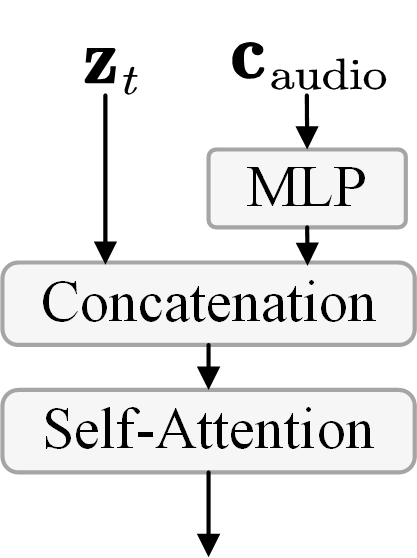
\includegraphics[width=\linewidth]{figs/AudioCondition/Audio_SA.png} 
                    \caption{}  
                    \label{fig:AudioConditionSA}  
                \end{subfigure}%
                \hfill
                \begin{subfigure}{0.3\linewidth} % 增加 subfigure 的宽度
                    \centering
                    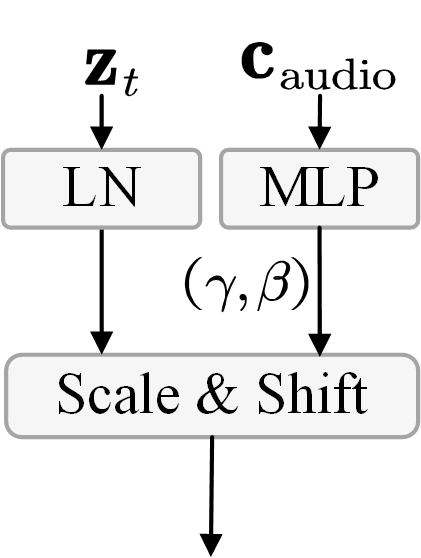
\includegraphics[width=\linewidth]{figs/AudioCondition/Audio_Ada.png}  
                    \caption{}  
                    \label{fig:AudioConditionAda}  
                \end{subfigure}%
                \hfill
                \begin{subfigure}{0.3\linewidth} % 增加 subfigure 的宽度
                    \centering
                    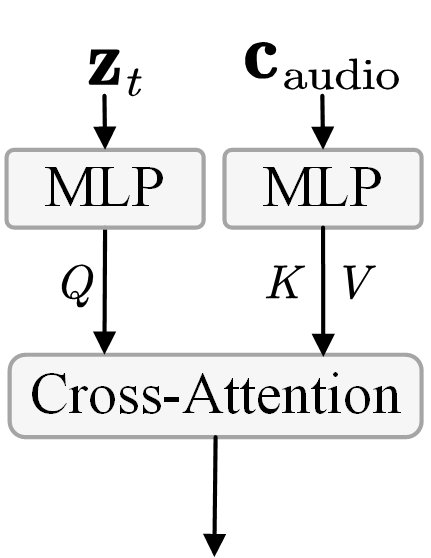
\includegraphics[width=\linewidth]{figs/AudioCondition/Audio_CA.png}  
                    \caption{}  
                    \label{fig:AudioConditionCA}  
                \end{subfigure}%
                \vspace{-1mm}
                \caption{Different strategies of audio conditioning. (a) self-attention; (b) adaptive norm; (c) cross-attention.}
                \label{fig:AudioCondition}
        \end{minipage}
        % \vspace{0.5cm} % 上下图片间距
        \begin{minipage}[b]{\textwidth} % 下方图
            \centering
            \begin{subfigure}{0.22\linewidth} % 增加 subfigure 的宽度
                \centering
                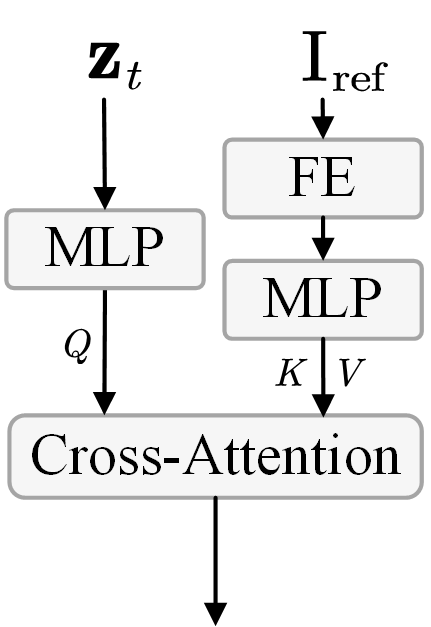
\includegraphics[width=0.95\linewidth]{figs/RefCondition/FE_CA.png} 
                \caption{}  
                \label{fig:RefConditionCA}  
            \end{subfigure}%
            \hfill
            \begin{subfigure}{0.22\linewidth} % 增加 subfigure 的宽度
                \centering
                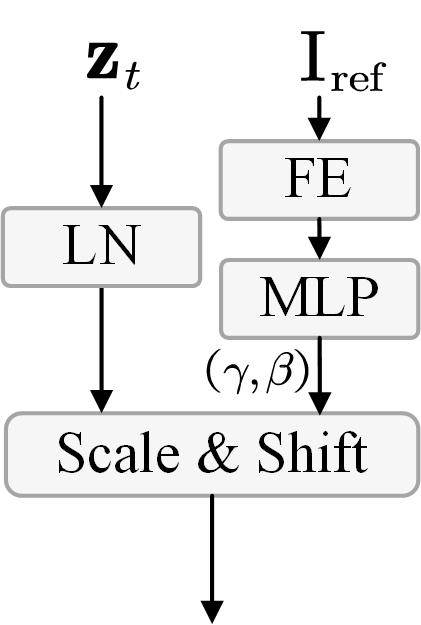
\includegraphics[width=0.95\linewidth]{figs/RefCondition/FE_Ada.png}  
                \caption{}  
                \label{fig:RefConditionAda}  
            \end{subfigure}%
            \hfill
            \begin{subfigure}{0.23\linewidth} % 增加 subfigure 的宽度
                \centering
                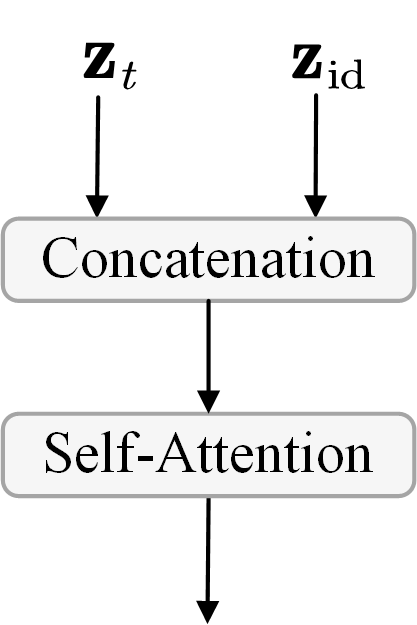
\includegraphics[width=0.95\linewidth]{figs/RefCondition/VAE_SA.png}  
                \caption{}  
                \label{fig:RefConditionVAESA}  
            \end{subfigure}%
            \hfill
            \begin{subfigure}{0.30\linewidth} % 增加 subfigure 的宽度
                \centering
                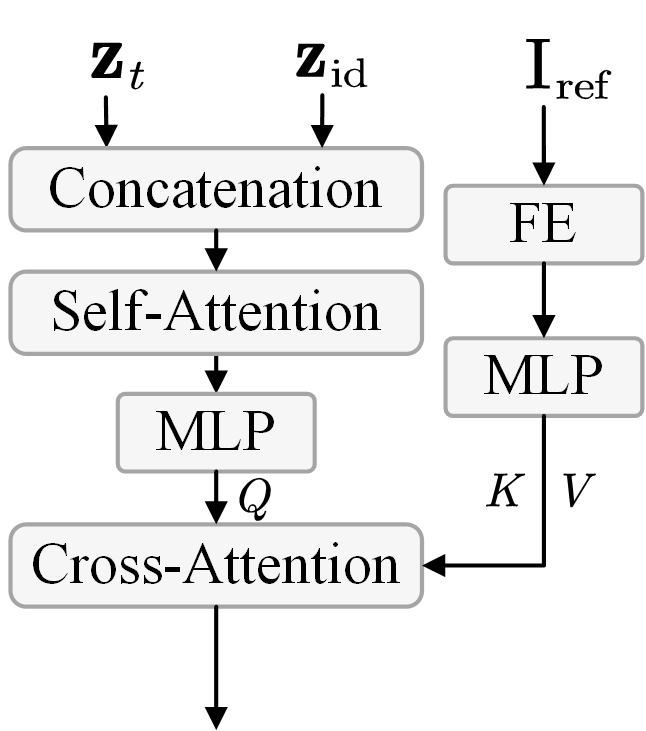
\includegraphics[width=\linewidth]{figs/RefCondition/VAE_CA.png}  
                \caption{}  
                \label{fig:RefConditionVAECA}  
            \end{subfigure}%
             \label{fig:RefCondition}
             \vspace{-1mm}
            \caption{{Different strategies of identity conditioning. FE refers to the face encoder. cross-attention demonstrates the best performance. (a) face attention; (b) face adaptive norm; (c) identity reference network; (d) face attention and identity reference network.}}
            \label{fig:IdCondition}
        \end{minipage}
    \end{minipage}
    % \vspace{5mm}
\end{figure*}


 
\section{Methodology}  
This methodology section systematically outlines the approaches employed in our study. 
Section~\ref{sec:baseline} describes the baseline transformer diffusion network, detailing its architecture and functionality. 
Section~\ref{sec:audio} focuses on the integration of speech audio conditions via a cross-attention mechanism. 
Section~\ref{sec:identity} discusses the implementation of the identity reference network, which is crucial for preserving facial identity coherence throughout extended video sequences. 
Section~\ref{sec:train} reviews the training and inference procedures used for the transformer diffusion network. 
Finally, Section~\ref{sec:data} details the comprehensive strategies for data sourcing and preprocessing.

\subsection{Baseline Transformer Diffusion Network}\label{sec:baseline}
\noindent\textbf{Baseline Network.}  
The CogVideoX model~\cite{yang2024cogvideox} serves as the foundational architecture for our transformer diffusion network, employing a 3D VAE for the compression of video data. 
In this framework, latent variables are concatenated and reshaped into a sequential format, denoted as \(\mathbf{z}_t\). 
Concurrently, the model utilizes the T5 architecture~\cite{raffel2023t5} to encode textual inputs into embeddings, represented as \(\mathbf{c}_{\text{text}}\). 
The combined sequences of video latent representations \(\mathbf{z}_t\) and textual embeddings \(\mathbf{c}_{\text{text}}\) are subsequently processed through an expert transformer network. 
To address discrepancies in feature space between text and video, we implement expert adaptive layer normalization techniques, which facilitate the effective utilization of temporal information and ensure robust alignment between visual and semantic data. 
Following this integration, a repair mechanism is applied to restore the original latent variable, after which the output is decoded through the 3D causal VAE decoder to reconstruct the video. 
Furthermore, the incorporation of 3D Rotational Positional Encoding (3D RoPE)~\cite{yang2024cogvideox} enhances the model's capacity to capture inter-frame relationships across the temporal dimension, thereby establishing long-range dependencies within the video framework.  

\noindent\textbf{Conditioning in Diffusion Transformer.}  
In addition to the textual prompt \(\mathbf{c}_{\text{text}}\), we introduce two supplementary conditions: the speech audio condition \(\mathbf{c}_{\text{audio}}\) and the identity appearance condition \(\mathbf{c}_{\text{id}}\).  

Within diffusion transformers, four primary conditioning mechanisms are identified: in-context conditioning, cross-attention, adaptive layer normalization (adaLN), and adaLN-zero~\cite{Peebles2022DiT}. 
Our investigation primarily focuses on cross-attention and adaptive layer normalization (adaLN). Cross-attention enhances the model's focus on conditional information by treating condition embeddings as keys and values, while latent representations serve as queries. 
Although adaLN is effective in simpler conditioning scenarios, it may not be optimal for more complex conditional embeddings that incorporate richer semantic details, such as sequential speech audio. Relevant comparative analyses will be elaborated upon in the experimental section.  

\subsection{Audio-Driven Transformer Diffusion}\label{sec:audio}
\noindent\textbf{Speech Audio Embedding.}  
To extract salient audio features for our proposed model, we utilize the wav2vec framework developed by Schneider et al.~\cite{schneider2019wav2vec}. The audio representation is defined as \(\mathbf{c}_{\text{audio}}\). 
Specifically, we concatenate the audio embeddings generated by the final twelve layers of the wav2vec network, resulting in a comprehensive semantic representation capable of capturing various audio hierarchies. 
This concatenation emphasizes the significance of phonetic elements, such as pronunciation and prosody, which are crucial as driving signals for character generation. 
To transform the audio embeddings obtained from the pretrained model into frame-specific representations, we apply three successive linear transformation layers, mathematically expressed as: $\mathbf{c}_{\text{audio}}^{(f)} = \mathcal{L}_3 \left( \mathcal{L}_2 \left( \mathcal{L}_1 \left( \mathbf{c}_{\text{audio}} \right) \right) \right)$, where \(\mathcal{L}_1\), \(\mathcal{L}_2\), and \(\mathcal{L}_3\) represent the respective linear transformation functions. This systematic approach ensures that the resulting frame-specific representations effectively encapsulate the nuanced audio features essential for the performance of our model.  

% \begin{figure}[th!]
% \vspace{-2mm}
%     \centering
%     \begin{subfigure}{0.3\linewidth} % 增加 subfigure 的宽度
%         \centering
%         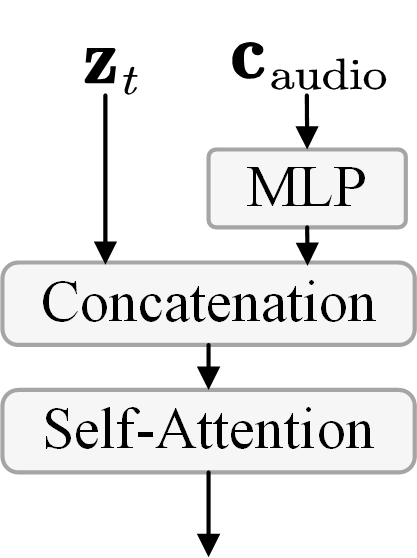
\includegraphics[width=\linewidth]{figs/AudioCondition/Audio_SA.png} 
%         \caption{Self-Attention}  
%         \label{fig:AudioConditionSA}  
%     \end{subfigure}%
%     \hfill
%     \begin{subfigure}{0.3\linewidth} % 增加 subfigure 的宽度
%         \centering
%         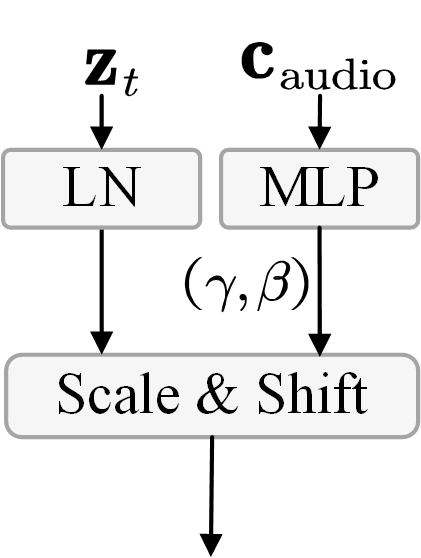
\includegraphics[width=\linewidth]{figs/AudioCondition/Audio_Ada.png}  
%         \caption{Adaptive Norm}  
%         \label{fig:AudioConditionAda}  
%     \end{subfigure}%
%     \hfill
%     \begin{subfigure}{0.3\linewidth} % 增加 subfigure 的宽度
%         \centering
%         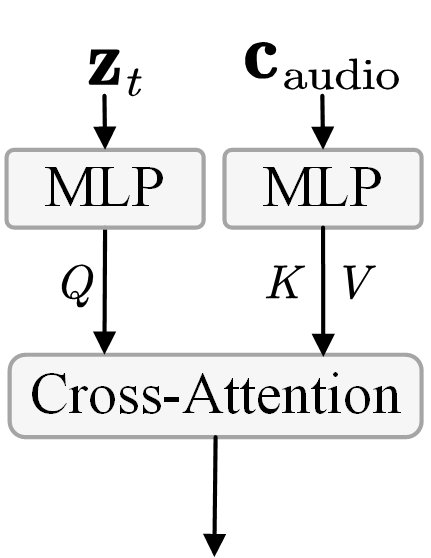
\includegraphics[width=\linewidth]{figs/AudioCondition/Audio_CA.png}  
%         \caption{Cross-Attention}  
%         \label{fig:AudioConditionCA}  
%     \end{subfigure}%
    
%     \caption{Different strategies of audio conditioning. Cross-Attention demonstrates the best performance.}
%     \label{fig:AudioCondition}
%     \vspace{-4mm}
% \end{figure}


\noindent\textbf{Speech Audio Conditioning.}  
We explore three fusion strategies---self-attention, adaptive normalization, and cross-attention---as illustrated in Figure~\ref{fig:AudioCondition} to integrate audio condition into the DiT-based video generation model. Our experiments show that the cross-attention strategy delivers the best performance in our model. For more details, please refer to Section~\ref{sec:ablationstudy}. 

Following this, 
 we integrate audio attention layers after each face-attention layer within the denoising network, employing a cross-attention mechanism that facilitates interaction between the latent encodings and the audio embeddings. 
Specifically, within the DiT block, the motion patches function as keys and values in the cross-attention computation with the hidden states \(\mathbf{z}_t\): $\mathbf{z}_t = \text{CrossAttention}(\mathbf{z}_t, \mathbf{c}_{\text{audio}}^{(f)})$. This methodology leverages the conditional information from the audio embeddings to enhance the coherence and relevance of the generated outputs, ensuring that the model effectively captures the intricacies of the audio signals that drive character generation.  




\subsection{Identity Consistent Transformer Diffusion}\label{sec:identity}

% \begin{figure}[th!]
%     \centering
%     \begin{subfigure}{0.22\linewidth} % 增加 subfigure 的宽度
%         \centering
%         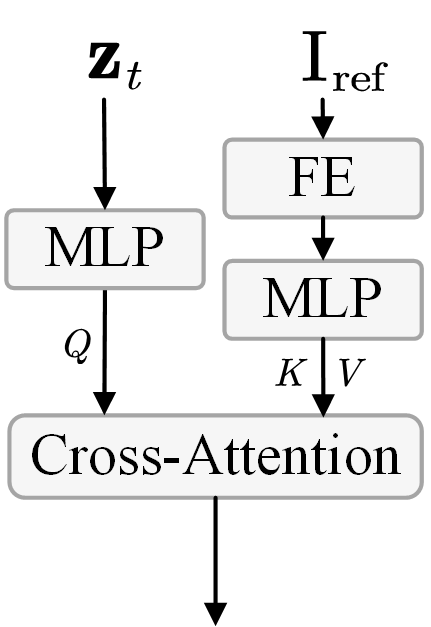
\includegraphics[width=0.95\linewidth]{figs/RefCondition/FE_CA.png} 
%         \caption{}  
%         \label{fig:RefConditionCA}  
%     \end{subfigure}%
%     \hfill
%     \begin{subfigure}{0.22\linewidth} % 增加 subfigure 的宽度
%         \centering
%         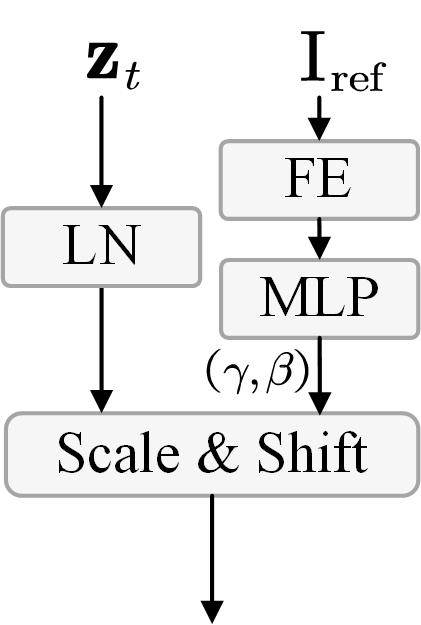
\includegraphics[width=0.95\linewidth]{figs/RefCondition/FE_Ada.png}  
%         \caption{}  
%         \label{fig:RefConditionAda}  
%     \end{subfigure}%
%     \hfill
%     \begin{subfigure}{0.23\linewidth} % 增加 subfigure 的宽度
%         \centering
%         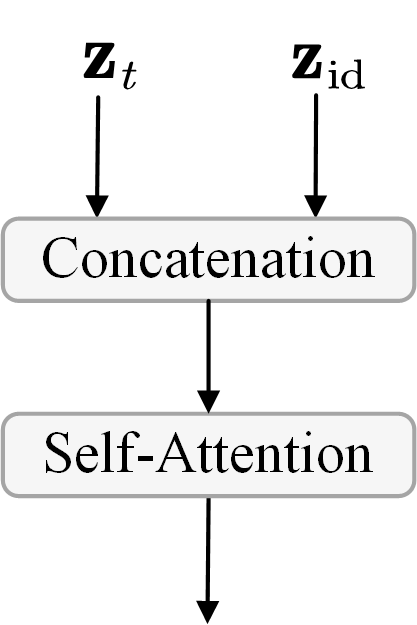
\includegraphics[width=0.95\linewidth]{figs/RefCondition/VAE_SA.png}  
%         \caption{}  
%         \label{fig:RefConditionVAESA}  
%     \end{subfigure}%
%     \hfill
%     \begin{subfigure}{0.30\linewidth} % 增加 subfigure 的宽度
%         \centering
%         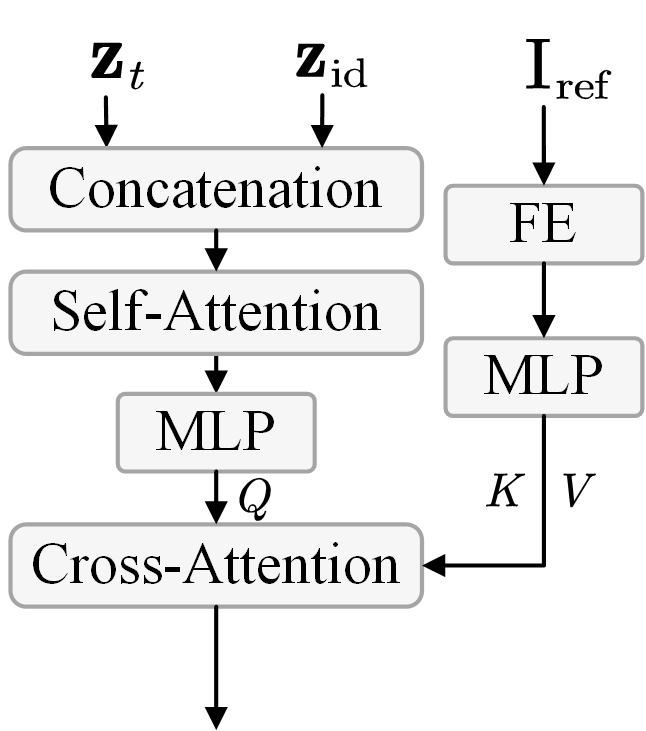
\includegraphics[width=\linewidth]{figs/RefCondition/VAE_CA.png}  
%         \caption{}  
%         \label{fig:RefConditionVAECA}  
%     \end{subfigure}%
%      \label{fig:RefCondition}
%     \caption{{Different strategies of identity conditioning. FE refers to the face encoder. Cross-Attention demonstrates the best performance. (a) Face attention; (b) Face adaptive norm; (c) Identity reference network; (d) Face attention and Identity reference network.}}

% \end{figure}



\noindent\textbf{Identity Reference Network.}  
Diffusion transformer-based video generation models encounter significant challenges in maintaining facial identity coherence, particularly as the length of the generated video increases. 
While incorporating speech audio embeddings as conditional features can establish a correspondence between audio speech and facial movements, prolonged generation often leads to rapid degradation of facial identity characteristics.  

To address this issue, we introduce a control condition within the existing diffusion transformer architecture to ensure long-term consistency of facial identity appearance. 
{We explore four strategies~(as shown in Figure~\ref{fig:IdCondition}) for appearance conditioning: 1) Face attention, where identity features are encoded by the face encoder and combined with a cross-attention module; 2) Face adaptive norm, which integrates features from the face encoder with an adaptive layer normalization technique; 3) Identity reference network, where identity features are captured by a 3D VAE and combined with some transformer layers; and 4) Face attention and Identity reference network, which encodes identity features using both the face encoder and 3D VAE, combining them with self-attention and cross-attention. Our experiments show that the combination with Face attention and Identity reference net achieves the best performance in our model. For further details, please refer to Section~\ref{sec:ablationstudy}. }

We treat a reference image as a single frame and input it into a causal 3D VAE to obtain latent features, which are then processed through a reference network consisting of 42 transformer layers. Mathematically, if \(\mathbf{I}_{\text{ref}}\) denotes the reference image, the encoder function of the 3D VAE is defined as: $\mathbf{z}_\text{id} = \mathcal{E}_{3D}(\mathbf{I}_{\text{ref}})$,
where \(\mathbf{z}_{\text{id}}\) represents the latent features associated with the reference image.  

During the operation of the reference network, we extract vision tokens from the input of the 3D full attention mechanism for each transformer layer, which serve as reference features \(\mathbf{z}_{\text{id}}\). These features are integrated into corresponding layers of the denoising network to enhance its capability, expressed as: $\mathbf{z}_{t, \text{enhanced}} = \text{SelfAttention}(\mathbf{z}_t, \mathbf{z}_{\text{id}}),$
where \(\mathbf{z}_t\) is the latent representation at time step \(t\). 
Given that both the reference network and denoising network leverage the same causal 3D VAE with identical weights and comprise the same number of transformer layers (42 layers in our implementation), the visual features generated from both networks maintain semantic and scale consistency. 
This consistency allows the reference network's features to incorporate the appearance characteristics of facial identity from the reference image while minimizing disruption to the original feature representations of the denoising network, thereby reinforcing the model's capacity to generate coherent and identity-consistent facial animations across longer video sequences.

\noindent\textbf{Temporal Motion Frames.}  
To facilitate long video inference, we introduce the last \(n\) frames of the previously generated video, referred to as motion frames, as additional conditions. Given a generated video length of \(L\) and the corresponding latent representation of \(l\) frames, we denote the motion frames as \(N\). 
The motion frames are processed through the 3D VAE to obtain \(n\) frames of latent codes. 
We apply zero padding to the subsequent \((l-n)\) frames and concatenate them with \(l\) frames of Gaussian noise. 
This concatenated representation is then patchified to yield vision tokens, which are subsequently input into the denoising network. By repeatedly utilizing motion frames, we achieve temporally consistent long video inference.



\subsection{Training and Inference}\label{sec:train}

\noindent\textbf{Training.}  
%The objective of the training process is to minimize the expected mean squared error between actual and predicted noise, framed by the loss function: $\mathcal{L} = \mathbb{E}_{\mathbf{z}_0, \mathbf{c}, \boldsymbol{\epsilon}, t} \left[ \omega(t) \left\| \boldsymbol{\epsilon} - \boldsymbol{\epsilon}_{\theta}(\mathbf{z}_t, t, \mathbf{c}) \right\|_2^2 \right]$, where \(\omega(t)\) serves as a weighting function to balance the loss in various time steps.  
The training process consists of two phases:

\textbf{(1) Identity Consistency Phase.} In this initial phase, we train the model to generate videos with consistent identity. The parameters of the 3D Variational Autoencoder (VAE) and face image encoder remain fixed, while the parameters of the 3D full attention blocks in both the reference and denoising networks, along with the face attention blocks in the denoising network, are updated during training. The model’s input includes a randomly sampled reference image from the training video, a textual prompt, and the face embedding. The textual prompt is generated using MiniCPM\cite{yao2024minicpm}, which describes human appearance, actions, and detailed environmental background. The face embedding is extracted via InsightFace\cite{insightface2024}. With these inputs, the model generates a video comprising 49 frames.

\textbf{(2) Audio-Driven Video Generation Phase.} In the second phase, we extend the training to include audio-driven video generation. We integrate audio attention modules into each transformer block of the denoising network, while fixing the parameters of other components and updating only those of the audio attention modules. Here, the model's input consists of a reference image, an audio embedding, and a textual prompt, resulting in a sequence of 49 video frames driven by audio.
% \text{}(1) In the first phase, we train the model to output videos with consistency of identity. The parameters of the 3D VAE and face image encoder are fixed, while the parameters of the 3D full attention in the reference network, composed of a series of transformer blocks, and those in the denoising network, including the 3D full attention and face attention, are updated through training. The model's input comprises a randomly sampled reference image from the training video, a textual prompt, and the face embedding obtained from the face encoder, with the output being a sequence of 49 frames of video. 
% (2) In the second phase, we train the model for audio-driven video generation. We insert audio attention modules into each transformer block of the denoising network, fixing the parameters of the other components and updating only those of the audio attention modules. The model's input consists of the reference image, input audio, and textual prompt, yielding a sequence of 49 frames of video.

\noindent\textbf{Inference.}  
%After training, new samples can be generated by initializing from a random Gaussian latent vector \(\mathbf{z}_T \sim \mathcal{N}(\mathbf{0}, \mathbf{I})\) and applying the iterative denoising process, defined as: $\mathbf{z}_{t-1} = \frac{1}{\sqrt{\alpha_t}} \left( \mathbf{z}_t - \frac{1 - \alpha_t}{\sqrt{1 - \bar{\alpha}_t}} \, \boldsymbol{\epsilon}_{\theta}(\mathbf{z}_t, t, \mathbf{c}) \right) + \sigma_t \mathbf{n}$, where \(\mathbf{n} \sim \mathcal{N}(\mathbf{0}, \mathbf{I})\) and \(t\) iterates from \(T\) to \(1\). The original image is reconstructed by decoding the final latent vector \(\mathbf{z}_0\) using the VAE decoder, yielding the generated output image represented as \(\mathbf{I} = \mathcal{D}(\mathbf{z}_0)\).  
During inference, the model receives a reference image, a segment of driving audio, a textual prompt, and motion frames as inputs. 
The model then generates a video that exhibits identity consistency and lip synchronization based on the driving audio. 
To produce long videos, we utilize the last two frames of the preceding video as motion frames, thereby achieving temporally consistent video generation.


% \begin{itemize}
%     \item \textbf{Extraction of Single-Speaker Video Clips:}
%     \begin{itemize}
%         \item \textbf{Shot Splitting and Re-encoding}: We employed scene detection and ffmpeg tools to split the videos into individual shots and re-encode them at a frame rate of 25 fps or lower, ensuring synchronization between audio and video data.
%         \item \textbf{Audio Processing}: Utilizing Ultimate Vocal Remover technology, we eliminated background music and environmental sounds from the videos, retaining only the vocal components. This step was crucial for ensuring alignment between audio embeddings and lip movements in the video.
%         \item \textbf{Segment Extraction}: Through the application of pyannote's speaker diarization and overlapped speech detection tools, we accurately extracted segments featuring a single speaker, ensuring that each video clip contained only one speaker's voice.
%     \end{itemize}

%     \item \textbf{Face and Camera Motion Filter:}
%     \begin{itemize}
%     \item **Facial Displacement Filter:** We employed InsightFace technology to calculate facial displacement in the videos, filtering out data where the facial displacement within a 17-frame window exceeded 50\% of the facial bounding box. This step ensured stable character movements and reduced facial blurriness due to rapid motion.
%     \item **Facial Rotation Filter:** Similarly, we utilized InsightFace technology to compute the facial rotation angles, particularly horizontal yaw, filtering out data with an average horizontal rotation exceeding 40°. This measure ensured that the faces in the videos were generally oriented towards the camera.
%     \item ** Camera Motion Filter:** Using CoTracker technology, we detected camera motion classifications in the videos and filtered out data exhibiting dynamic camera movements to minimize interference from moving backgrounds.
%     \item **Audio Lip Sync Filter:** We employed SyncNet technology to compute the audio-visual synchronization scores of the videos, filtering out data with scores below 5.0.
%     \end{itemize}
%     \item \textbf{Data Post-processing:}
%     \begin{itemize}
%         \item **Video Cropping:** Based on the facial positions detected in the previous steps, we cropped the videos into segments with a 3:2 aspect ratio to meet the model's input requirements.
%         \item **Facial Encoding:** A random frame's face was selected, and InsightFace technology was utilized to encode it into embeddings, providing essential facial feature information for the model.
%         \item **Audio Encoding:** The audio from the videos was extracted and encoded into embeddings using Wav2Vec2 technology, facilitating the injection of audio conditions during model training.
%     \end{itemize}
% \end{itemize}

    % \item \textbf{Facial Displacement Calculation:} We employed insightface technology to calculate facial displacement in the videos, filtering out data where the facial displacement within a 17-frame window exceeded 50\% of the facial bounding box. This step ensured stable character movements and reduced facial blurriness due to rapid motion.
    
    % \item \textbf{Facial Rotation Angle Calculation:} Similarly, we utilized insightface technology to compute the facial rotation angles, particularly horizontal yaw, filtering out data with an average horizontal rotation exceeding 40°. This measure ensured that the faces in the videos were generally oriented towards the camera.
    
    % \item \textbf{Camera Motion Classification Detection:} Using CoTracker technology, we detected camera motion classifications in the videos and filtered out data exhibiting dynamic camera movements to minimize interference from moving backgrounds.
    
    % \item \textbf{SyncNet Score Calculation:} We employed SyncNet technology to compute the audio-visual synchronization scores of the videos, filtering out data with scores below 5.0.


\begin{figure*}[t]
    \centering
    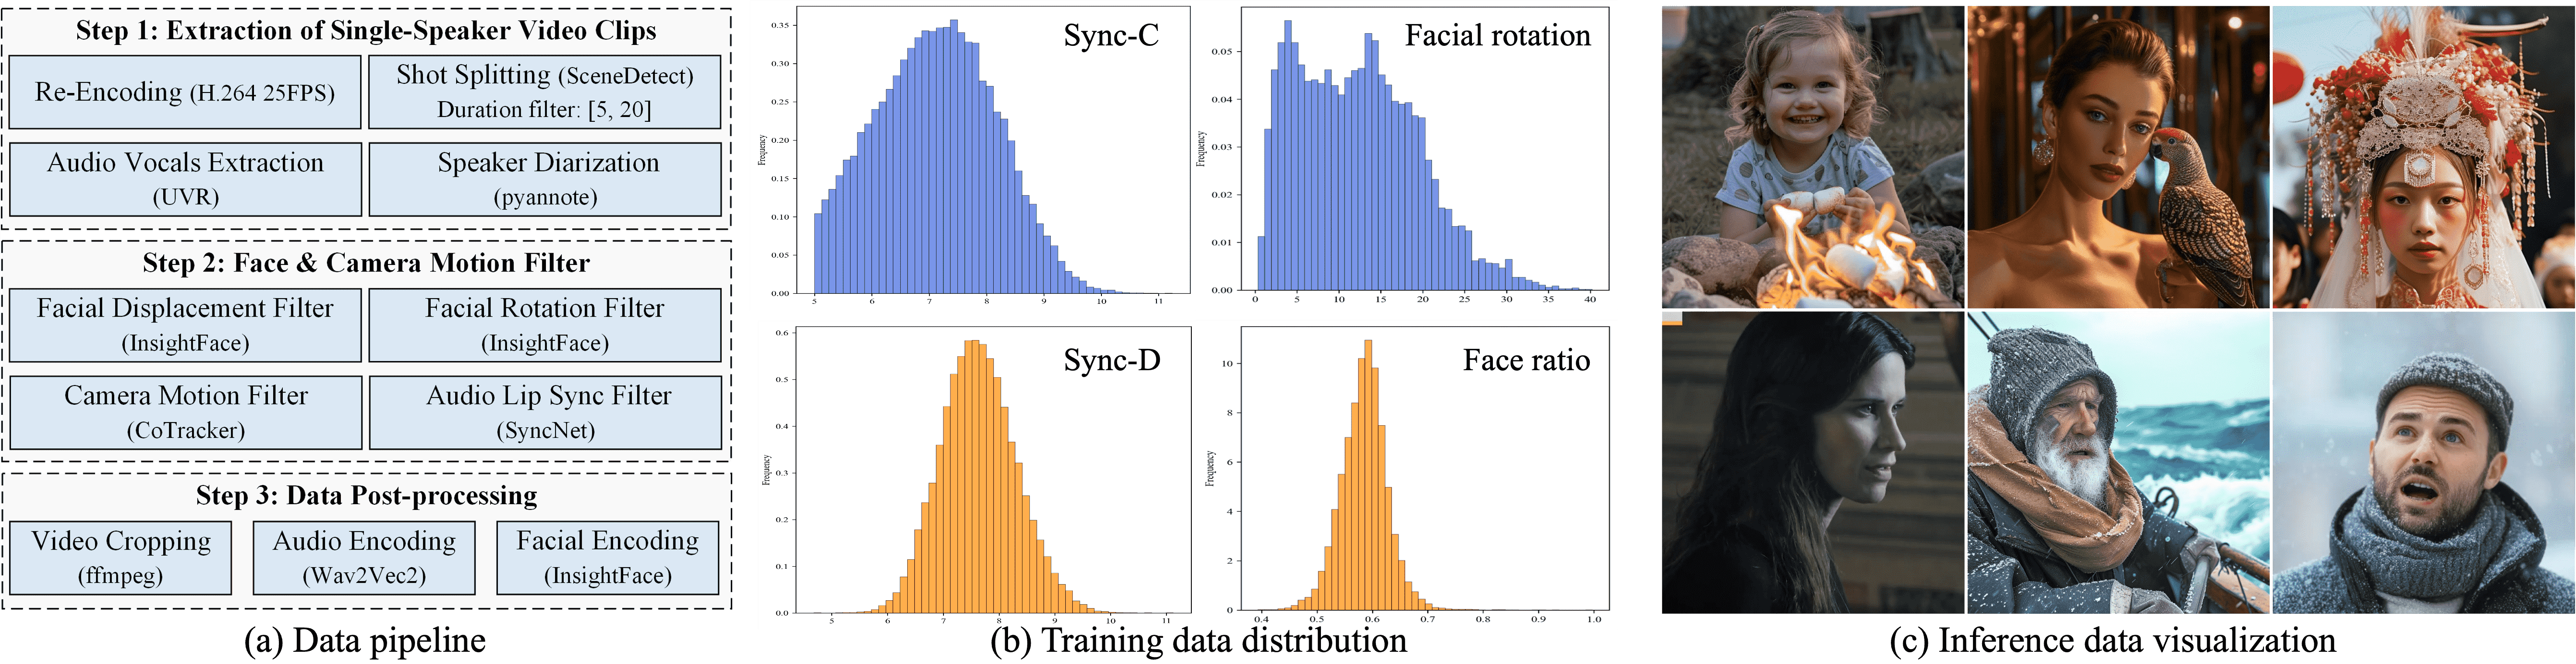
\includegraphics[width=\linewidth]{figs/dataset_comp.png}
    \vspace{-7mm}
    \caption{{
Illustration of the dataset, including the flow of data processing, data distribution across different metric, and the visualization of some representative portrait images for inference.}}
    \label{fig:data_statistics}
    % \vspace{-4mm}
\end{figure*}


\subsection{Dataset}\label{sec:data}



In this section, we will give a detailed introduction of our data curation, including data sources, filtering strategy and data statistics.
Figure~\ref{fig:data_statistics} shows the data pipeline and the statistical analysis of the final data.

\noindent\textbf{Data Sources}
The training data used in this work is prepared from three distinct sources to ensure diversity and generalization. Specifically, the sources are: (1) HDTF dataset~\cite{zhang2021flow}, which contains 8 hours of raw video footage; (2) YouTube data, which consists of 1,200 hours of public raw videos; (3) a large scale movie dataset, which contains film videos of 2,346 hours. 
Our dataset contains a large scale of human identities and, however, we find that YouTube and movie dataset contains  a large amount of noised data. Therefore, we design a data curation pipeline as follows to construct a high-quality and diverse talking dataset, as shown in Figure~\ref{fig:data_statistics}(a).

% \begin{itemize}

%     \item \textbf{HDTF Dataset:} this open-source Talking Face video dataset provides 8 hours of raw video footage. After extensive cleaning and preprocessing, 6 hours of high-quality data are curated for model training.
    
%     \item \textbf{YouTube Data:} We collect 1,200 hours of video data from YouTube, and apply a thorough cleaning process that involved removing duplicates, low-quality videos, and irrelevant content. Finaly, 72 hours of high-quality video are left for training.
    
%     \item \textbf{Film Data:}  To diversify the dataset, we collect and construct a large scale movie video dataset, which contains 2,346 hours. After data curation, 53 hours of video data are retained.
% \end{itemize}



\noindent\textbf{Video Filtering.}
During the data pre-processing phase, we implement a series of meticulous filtering steps to ensure the quality and applicability of the dataset. The workflow includes three stages: extraction of single-speaker, motion filter and post-processing. Firstly, we select video of single-speaker. This stage aims to clean the video content to solve camera shot, background noise, etc, using existing tools~\cite{Plaquet23,Bredin23}. After that, we apply several filtering techniques to ensure the quality of head motion, head pose, camera motion, etc~\cite{karaev23cotracker,karaev24cotracker3,Chung16a}. In this stage, we compute all metric scores for each clip, therefore, we can flexibly adjust data screening strategies to satisfy different data requirement of our multiple training stages or strategies. Finally, based on the facial positions detected in previous steps, we crop the videos to a 3:2 aspect ratio to meet the model's input requirements. We then select a random frame from each video and use InsightFace~\cite{ren2023pbidr} to encode the face into embeddings, providing essential facial feature information for the model. Additionally, we extract the audio from the videos and encode it into embeddings using Wav2Vec2 model~\cite{baevski2020wav2vec}, facilitating the incorporation of audio conditions during model training.

\noindent\textbf{Data Statistics.}
Following the data cleaning and filtering processes, we conducted a detailed analysis of the final dataset to assess its quality and suitability for the intended modeling tasks. Finally, our training data contains about 134 hours of videos, including 6 hours of high-quality data from HDTF dataset, 72 hours of YouTube videos, and 56 hours of movie videos. Figure~\ref{fig:data_statistics}(b) also shows other statistics, such as Lip Sync score~(Sync-C and Sync-D), face rotation, face ratio~(the ratio of face height to video height).
%As can be seen in Fig~\ref{fig:data_statistics}b, our dataset has a large.





\begin{table*}[t!]
    \centering
    % 第一个表格
    \begin{minipage}{0.25\textwidth}
        \centering
        \resizebox{\textwidth}{!}{
        \begin{tabular}{c|c|c|c|c}
        \toprule
        \ &
          \multicolumn{1}{c|}{FID$\downarrow$} &
          \multicolumn{1}{c|}{FVD$\downarrow$} &
          \multicolumn{1}{c|}{Sync-C$\uparrow$} &
          \multicolumn{1}{c}{Sync-D$\downarrow$} \\ 
          \midrule
        SadTalker~\cite{zhang2022sadtalker}   & 22.340 & 203.860 & \textbf{7.885} & \textbf{7.545}  \\
        DreamTalk~\cite{ma2023dreamtalk}      & 78.147 & 790.660 & 6.376 & 8.364  \\
        AniPortrait~\cite{wei2024aniportrait} & 26.561 & 234.666 & 4.015 & 10.548  \\
        Hallo~\cite{xu2024hallo}              & 20.545 & 173.497 & 7.750 & 7.659  \\
        Ours                                  & \textbf{20.359} & \textbf{160.838} & 7.252 & 8.106  \\ 
        \midrule
        Real video                            & - & - & 8.700 & 6.597 \\ 
        \bottomrule
        \end{tabular}}
        \vspace{-2mm}
        \caption{Comparison with the other methods on HDTF dataset.} 
        \label{tab:comp_hdtf}
    \end{minipage}
    \hfill
    % 第二个表格
    \begin{minipage}{0.30\textwidth}
        \centering
        \resizebox{\textwidth}{!}{
        \begin{tabular}{c|c|c|c|c|c}
        \toprule
            \ &
              \multicolumn{1}{c|}{FID$\downarrow$} &
              \multicolumn{1}{c|}{FVD$\downarrow$} &
              \multicolumn{1}{c|}{Sync-C$\uparrow$} &
              \multicolumn{1}{c|}{Sync-D$\downarrow$} &
              \multicolumn{1}{c}{E-FID$\downarrow$} \\ 
              \midrule
            SadTalker~\cite{zhang2022sadtalker}   & 50.015 & 471.163 & 6.922 & \textbf{7.921} & 95.194 \\
            DreamTalk~\cite{ma2023dreamtalk}      & 109.011 & 988.539 & 5.709 & 8.743 & 153.450 \\
            AniPortrait~\cite{wei2024aniportrait} & 46.915 & 477.179 & 2.853 & 11.709 & 88.986 \\
            Hallo~\cite{xu2024hallo}              & 44.578 & 377.117 & \textbf{7.191} & 7.984 & 78.495 \\
            Ours                                  & \textbf{43.271} & \textbf{355.272} & 6.527 & 9.113 & \textbf{71.210} \\ 
            \midrule
            Real video                            & - & - & 7.372 & 7.518 & - \\ 
            \bottomrule
        \end{tabular}}
        \vspace{-2mm}
        \caption{Comparison with other methods on Celeb-V dataset.}
        \label{tab:comp_celebv}
    \end{minipage}
    \hfill
    % 第三个表格
    \begin{minipage}{0.39\textwidth}
        \centering
        \resizebox{\textwidth}{!}{
        \begin{tabular}{c|c|c|c|c|c|c}
        \toprule
        \ &
          \multicolumn{1}{c|}{Sync-C$\uparrow$} &
          \multicolumn{1}{c|}{Sync-D$\downarrow$} &
          \makecell{Subject\\Dynamic$\uparrow$} &
          \makecell{Background\\Dynamic$\uparrow$} &
          \makecell{Subject\\FVD$\downarrow$} &
          \makecell{Background\\FVD$\downarrow$} \\ 
          \midrule   
        SadTalker~\cite{zhang2022sadtalker}  & 3.845           & 10.378         & 2.953   & 0.220 & 470.377 &313.758 \\
        DreamTalk~\cite{ma2023dreamtalk}     & 4.498           & 11.005         & 6.958   & 1.806 & 835.480 &744.177 \\
        AniPortrait~\cite{wei2024aniportrait}&	1.685           & 12.025        & 3.351  & 1.769 & 473.173 & 302.716 \\
        Hallo~\cite{xu2024hallo}             & 4.654           & 10.202         & 5.268   & 1.272 & 394.627 & 291.052 \\
        Ours                                 & \textbf{6.154}  & \textbf{8.574} & 
         \textbf{13.286}  & \textbf{4.481} & \textbf{359.493} &\textbf{248.283} \\ 
        \bottomrule
        \end{tabular}}
        \vspace{-2mm}
        \caption{Comparison with other methods on our proposed wild dataset.}
        \label{tab:comparison_wild}
    \end{minipage}
    \vspace{2mm}
\end{table*}


\begin{figure*}[t!]
    \centering
    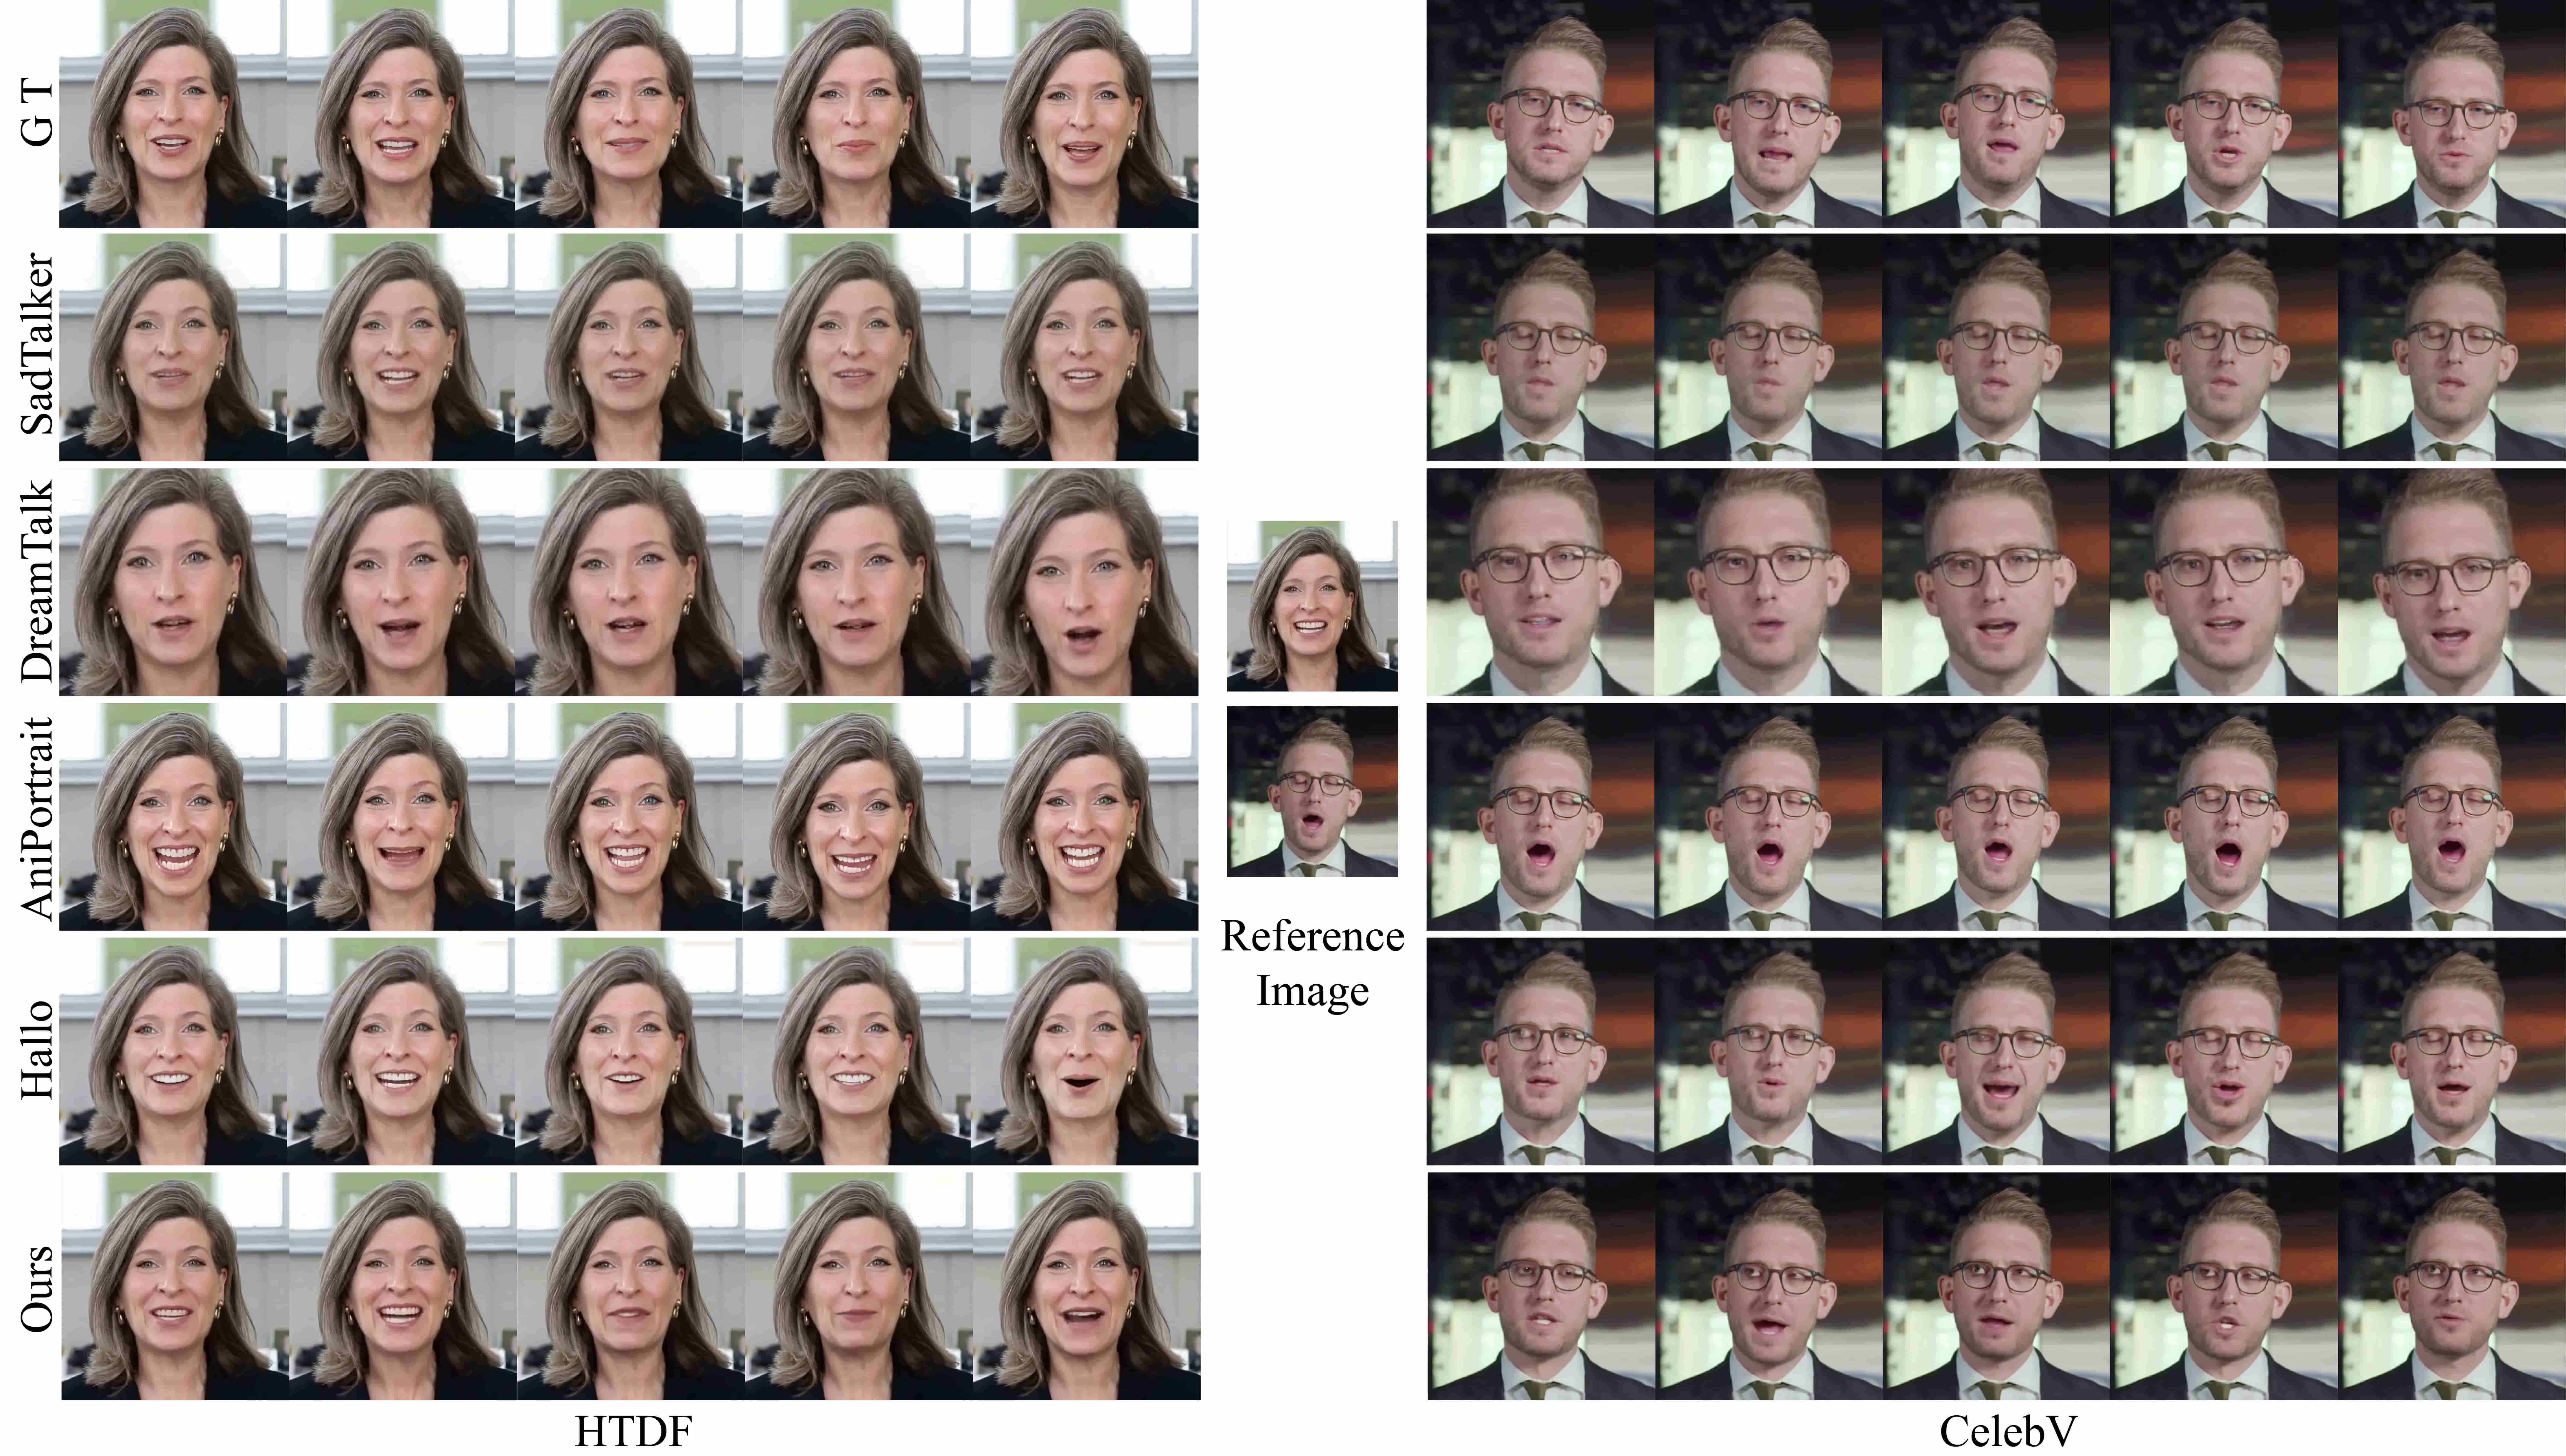
\includegraphics[width=\linewidth]{figs/HTDF_CelebV_comp.jpg}
    \vspace{-6mm}
    \caption{Qualitative comparison on the HTDF~(left) and CelebV~(right) data-set.}
    \vspace{-2mm}
    \label{fig:hdtf}
\end{figure*}





% \begin{figure}[th!]
%     \centering
%     % Creates an empty box with dimensions
%     % \rule{\linewidth}{0.5\linewidth}
%     \includegraphics[width=1\linewidth]{figs/comparisn_of_audio_conditioning2.pdf}
%     \caption{Qualitative comparison of different strategies for audio conditioning.}
%     \label{fig:comparisn_of_audio_conditioning2}
%     \vspace{-4mm}
% \end{figure}

% \begin{figure}[th!]
%     \centering
%     % Creates an empty box with dimensions
%     % \rule{\linewidth}{0.5\linewidth}
%      \includegraphics[width=1\linewidth]{figs/Comparison_of_the_appearance_reference_network.pdf}
%     \caption{ Qualitative comparison of different strategies for indentity conditioning.}
%     \label{fig:Comparison_of_the_appearance_reference_network}
% \end{figure}

\section{Experiment}
\subsection{Experimental Setups}
% \noindent\textbf{Comparison on dynamic scene scenarios.}

\noindent\textbf{Implementation.}
% {The model was trained using 64 NVIDIA A100 GPUs. In addition to training, all experiments were conducted on a GPU server equipped with 8 NVIDIA A100 GPUs. The first and second stages of the model were trained 20,000 steps respectively. During training, the batch size of each GPU was 1, and the learning rate was set to 1e-5. The resolution of the training video is 480 x 720, and it can generate a video with 49 frames at a time. In the training process, the audio embedding is dropped with a probability of 0.05, and the motion frames are randomly masked with a probability of 0.25.}
We initialize the identity reference and denoising networks with weights derived from CogVideoX-5B-I2V\cite{yang2024cogvideox}. During both training phases, we employ the v-prediction diffusion loss\cite{salimans2022progressive} for optimization. Each training phase comprises 20,000 steps, utilizing 64 NVIDIA H100 GPUs. The batch size per GPU is set to 1, with a learning rate of \(480 \times 720\) pixels. To enhance video generation variability, the reference image, guidance audio and textual prompt are dropped with a probability of 0.05 during training.

\noindent\textbf{Evaluation Metrics.}
We employed a range of evaluation metrics for generated videos across benchmark datasets, including HDTF~\cite{zhang2021flow} and Celeb-V~\cite{zhu2022celebvhq}. 
These metrics comprise Fréchet Inception Distance (FID)~\cite{Seitzer2020FID}, Fréchet Video Distance (FVD)~\cite{unterthiner2018towards}, Synchronization-C (Sync-C)~\cite{Chung16a}, Synchronization-D (Sync-D)~\cite{Chung16a}, and E-FID~\cite{tian2024emo}. 
FID and FVD quantify the similarity between generated images and real data, while Sync-C and Sync-D assess lip synchronization accuracy. E-FID evaluates the image quality based on features extracted from the Inception network.
Besides, we introduced VBench~\cite{huang2023vbench} metrics to enhance evaluation, focusing on dynamic degree and subject consistency. 
% Background consistency is evaluated via CLIP feature similarity, assessing the temporal stability of backgrounds. 
%Temporal flickering is quantified by mean absolute differences in static frames, while motion smoothness is analyzed using motion priors from a video frame interpolation model. 
Dynamic degree is measured using RAFT~\cite{teed2020raft} to quantify the extent of motion in generated videos, providing a comprehensive assessment of temporal quality.
Subject consistency is measured through DINO~\cite{caron2021emerging} feature similarity, ensuring uniformity of a subject's appearance across frames. 


\noindent\textbf{Baseline Approaches.}
We considered several representative audio-driven talking face generation methods for comparison, all of which have publicly available source code or implementations. These methods include SadTalker~\cite{zhang2022sadtalker}, DreamTalk~\cite{ma2023dreamtalk}, AniPortrait~\cite{wei2024aniportrait}, and Hallo~\cite{xu2024hallo,cui2024hallo2}. 
The selected approaches encompass both GANs and diffusion models, as well as techniques utilizing intermediate facial representations alongside end-to-end frameworks. 
This diversity in methodologies allows for a comprehensive evaluation of the effectiveness of our proposed approach compared to existing solutions.

% Subject consistency is measured through DINO feature similarity, ensuring uniformity of a subject's appearance across frames. 
% Background consistency is evaluated via CLIP feature similarity, assessing the temporal stability of backgrounds. 
%Temporal flickering is quantified by mean absolute differences in static frames, while motion smoothness is analyzed using motion priors from a video frame interpolation model. 
%Dynamic degree is measured using RAFT to quantify the extent of motion in generated videos, providing a comprehensive assessment of temporal quality.

%\noindent\textbf{Datasets} Our dataset comprises HDTF~\cite{zhang2021flow} as well as additional data sourced from the Internet. In order to build a dataset of both high quality and diversity, we have designed a comprehensive data curation pipeline capable of processing a wide variety of Internet videos, including YouTube and movie clips. Specifically, we collected 1200 hours of YouTube videos and 2346 hours of movie footage, from which we curated 128 hours of high-quality video clips. The details of the pipeline and related statistics are presented in Figure~\ref{fig:data_statistics}. For further discussions, please refer to the Appendix.





\subsection{Comparison with State-of-the-art}

\noindent\textbf{Comparison on HDTF and Celeb-V Dataset.}
{As shown in Table~\ref{tab:comp_hdtf} and ~\ref{tab:comp_celebv}, our method achieves best results on FID, FVD on both datasets. Although our approach shows some disparity compared to the state-of-the-art in lip synchronization, it still demonstrates promising results as illustrated in Figure~\ref{fig:hdtf}. This is because, to generate animated portraits from different perspectives, our training data primarily consists of talking videos with significant head and body movements, as well as diverse dynamic scenes, unlike static scenes with minimal motion. While this may lead to some performance degradation on lip synchronization, it better reflects realistic application scenarios. }
%We find that large head pose diversity~(such as large head turning) and head motion may lead to the degeneration. 

%\noindent\textbf{Comparison on Celeb-V Dataset.}
%\textcolor{red}{Table~\ref{tab:comp_celebv} presents quantitative comparison on CelebV dataset. }
% and qualitative 



\noindent\textbf{Comparison on Wild Dataset.} 
To effectively demonstrate the performance of the general talking portrait video generation, we carefully collect 34 representative cases for evaluation. This dataset consists of portrait images with various head proportions, head poses, static and dynamic scenes and complex headwears and clothing. To achieve comprehensive assessment, we evaluate the performance on lip synchronization~(Sync-C and Sync-D), motion strength (subject and background dynamic degree) and  video quality~(subject and background FVD).
As shown in Table~\ref{tab:comparison_wild}, our method generates videos with largest head and background dynamic degree~(13.286 and 4.481) while keeping lip synchronization of highest accuracy. 

Figure~\ref{fig:portrait_complex_face} provides a qualitative comparison of different portrait methods on a ``wild" dataset. The results reveal that other methods struggle to animate side-face portrait images, often resulting in static poses or facial distortions. Additionally, these methods tend to focus solely on animating the face, overlooking interactions with other objects in the foreground---such as the dog next to the elderly, or the dynamic movement of the background---like the ostrich behind the girl. In contrast, as shown in Figure~\ref{fig:ComplexScenes} our method produces realistic portraits with diverse orientations and complex foreground and background scenes.



\begin{figure*}[t!]
    \hspace{-2.5mm}
    \centering    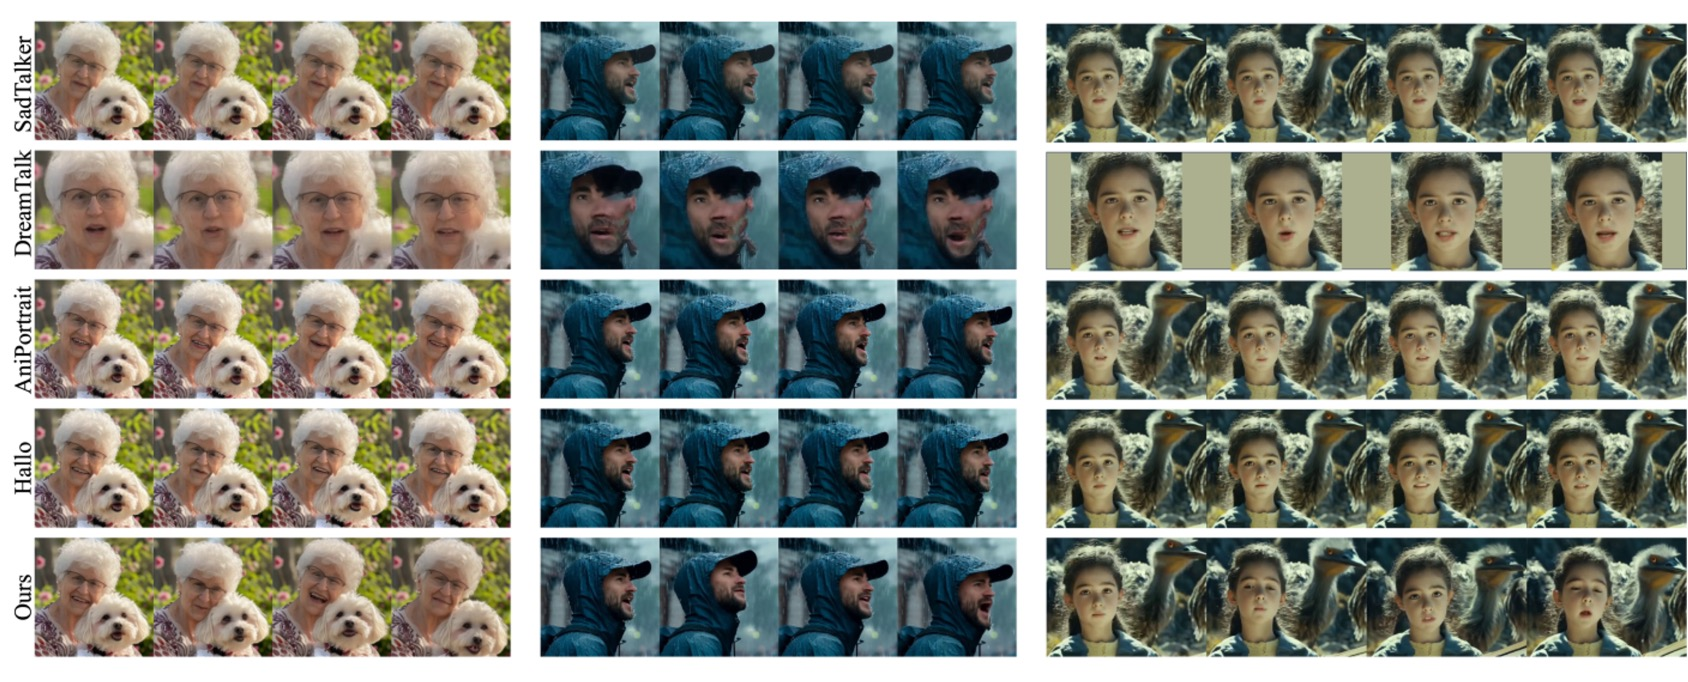
\includegraphics[width=1.01\linewidth]{figs/method_comparison3_2.jpg}
    \vspace{-7mm}
    \caption{Complex facial identity with dynamic accessories subjects and different pose orientation.}
    
    \label{fig:portrait_complex_face}
    \vspace{2mm}
\end{figure*}

\begin{figure*}[t!]
    \centering
    \includegraphics[width=1.0\linewidth]{figs/ComplexScenes.jpg}
    \vspace{-6mm}
    \caption{Complex scenes with dynamic foreground or background and various head poses.}
    \label{fig:ComplexScenes}
    \vspace{-2mm}
\end{figure*}










\subsection{Ablation Study and Discussion}
\label{sec:ablationstudy}
\noindent\textbf{Audio Conditioning.} {Table~\ref{tab:audio_injection} and Figure~\ref{fig:comparisn_of_audio_conditioning2} illustrate the effects of various strategies for incorporating audio conditioning. The results demonstrate that using cross-attention to integrate audio improves lip synchronization by enhancing the local alignment between visual and audio features, particularly around the lips. This is evident from the improvements in Sync-C and Sync-D, and it also contributes to a degree of enhancement in video quality.}

\noindent\textbf{Identity Reference Network.} {
Table~\ref{tab:identity_preserve} and Figure~\ref{fig:Comparison_of_the_appearance_reference_network} evaluate different identity conditioning strategies.  The results indicate that without an identity condition, the model fails to preserve the portrait appearance. When using face embedding alone, the model introduces blur and distortion, as it focuses solely on facial features and disrupts the global visual context. To address this, we introduce an identity reference network to preserve global features while making facial motion more controllable through identity-based facial embeddings. Thus, the proposed method achieves a lower FID of 23.458 and FVD of 242.602, while maintaining lip synchronization.
}

\noindent\textbf{Temporal Motion Frames.} {Table~\ref{tab:motion_frame_num} presents an analysis of varying temporal motion frames. One motion frame achieves the highest Sync-C score (6.889) and the lowest Sync-D score (8.695), indicating substantial lip synchronization.}

% \subsection{Limitations and Future Works}
% \textcolor{red}{This paper presents advancements in wild portrait image animation with different perspective and complex scenes, there exist several limitations that necessitate further exploration and consideration. (1)...}
% \begin{table}[]
% \centering
% \footnotesize
% \begin{tabular}{lc|l|l|l|l|l|l}
% \cline{2-8}
%  &
%   FD & PG &
%   \multicolumn{1}{c|}{FID$\downarrow$} &
%   \multicolumn{1}{c|}{FVD$\downarrow$} &
%   \multicolumn{1}{c|}{Sync-C$\uparrow$} &
%   \multicolumn{1}{c|}{Sync-D$\downarrow$} &
%   \multicolumn{1}{c}{E-FID$\downarrow$} \\ \cline{2-8} 
%  &            &            & - & - & - & - & - \\
%  & \checkmark &            & - & - & - & - & - \\
%  &            & \checkmark & - & - & - & - & - \\
%  & \checkmark & \checkmark & - & - & - & - & - \\ \cline{2-8} 
% \end{tabular}
% \caption{Ablation on augmentation for id preservation. FD: Frame drop; PG: Pixel Gaussian}
% \label{tab:abl_id_augment}
% \end{table}


\noindent
\textbf{CFG Scales for Diffusion Model.}  
Table~\ref{tab:abalation_cfg} provides a quantitative analysis of video generations using various CFG scales for audio, text, and reference images. A comparison between the second and fourth rows demonstrates that increasing the audio CFG scale enhances the model's ability to synchronize lip movements. The text CFG scale significantly influences the video’s dynamism, as indicated in the first three rows, where both the subject's and the background's dynamics increase with higher text CFG scales. Conversely, the reference image CFG scale primarily governs the subject's appearance; higher values improve subject consistency, as illustrated by the second and fifth rows. Among the tested configurations, setting \(\lambda_a=3.5\), \(\lambda_t=3.5\), and \(\lambda_i=1.0\) yields a balanced performance. This interplay between visual fidelity and dynamics underscores the effectiveness of CFG configurations in generating realistic portrait animations.


\begin{figure*}[!t]
    \centering
    \begin{minipage}{0.48\linewidth}
        \centering
        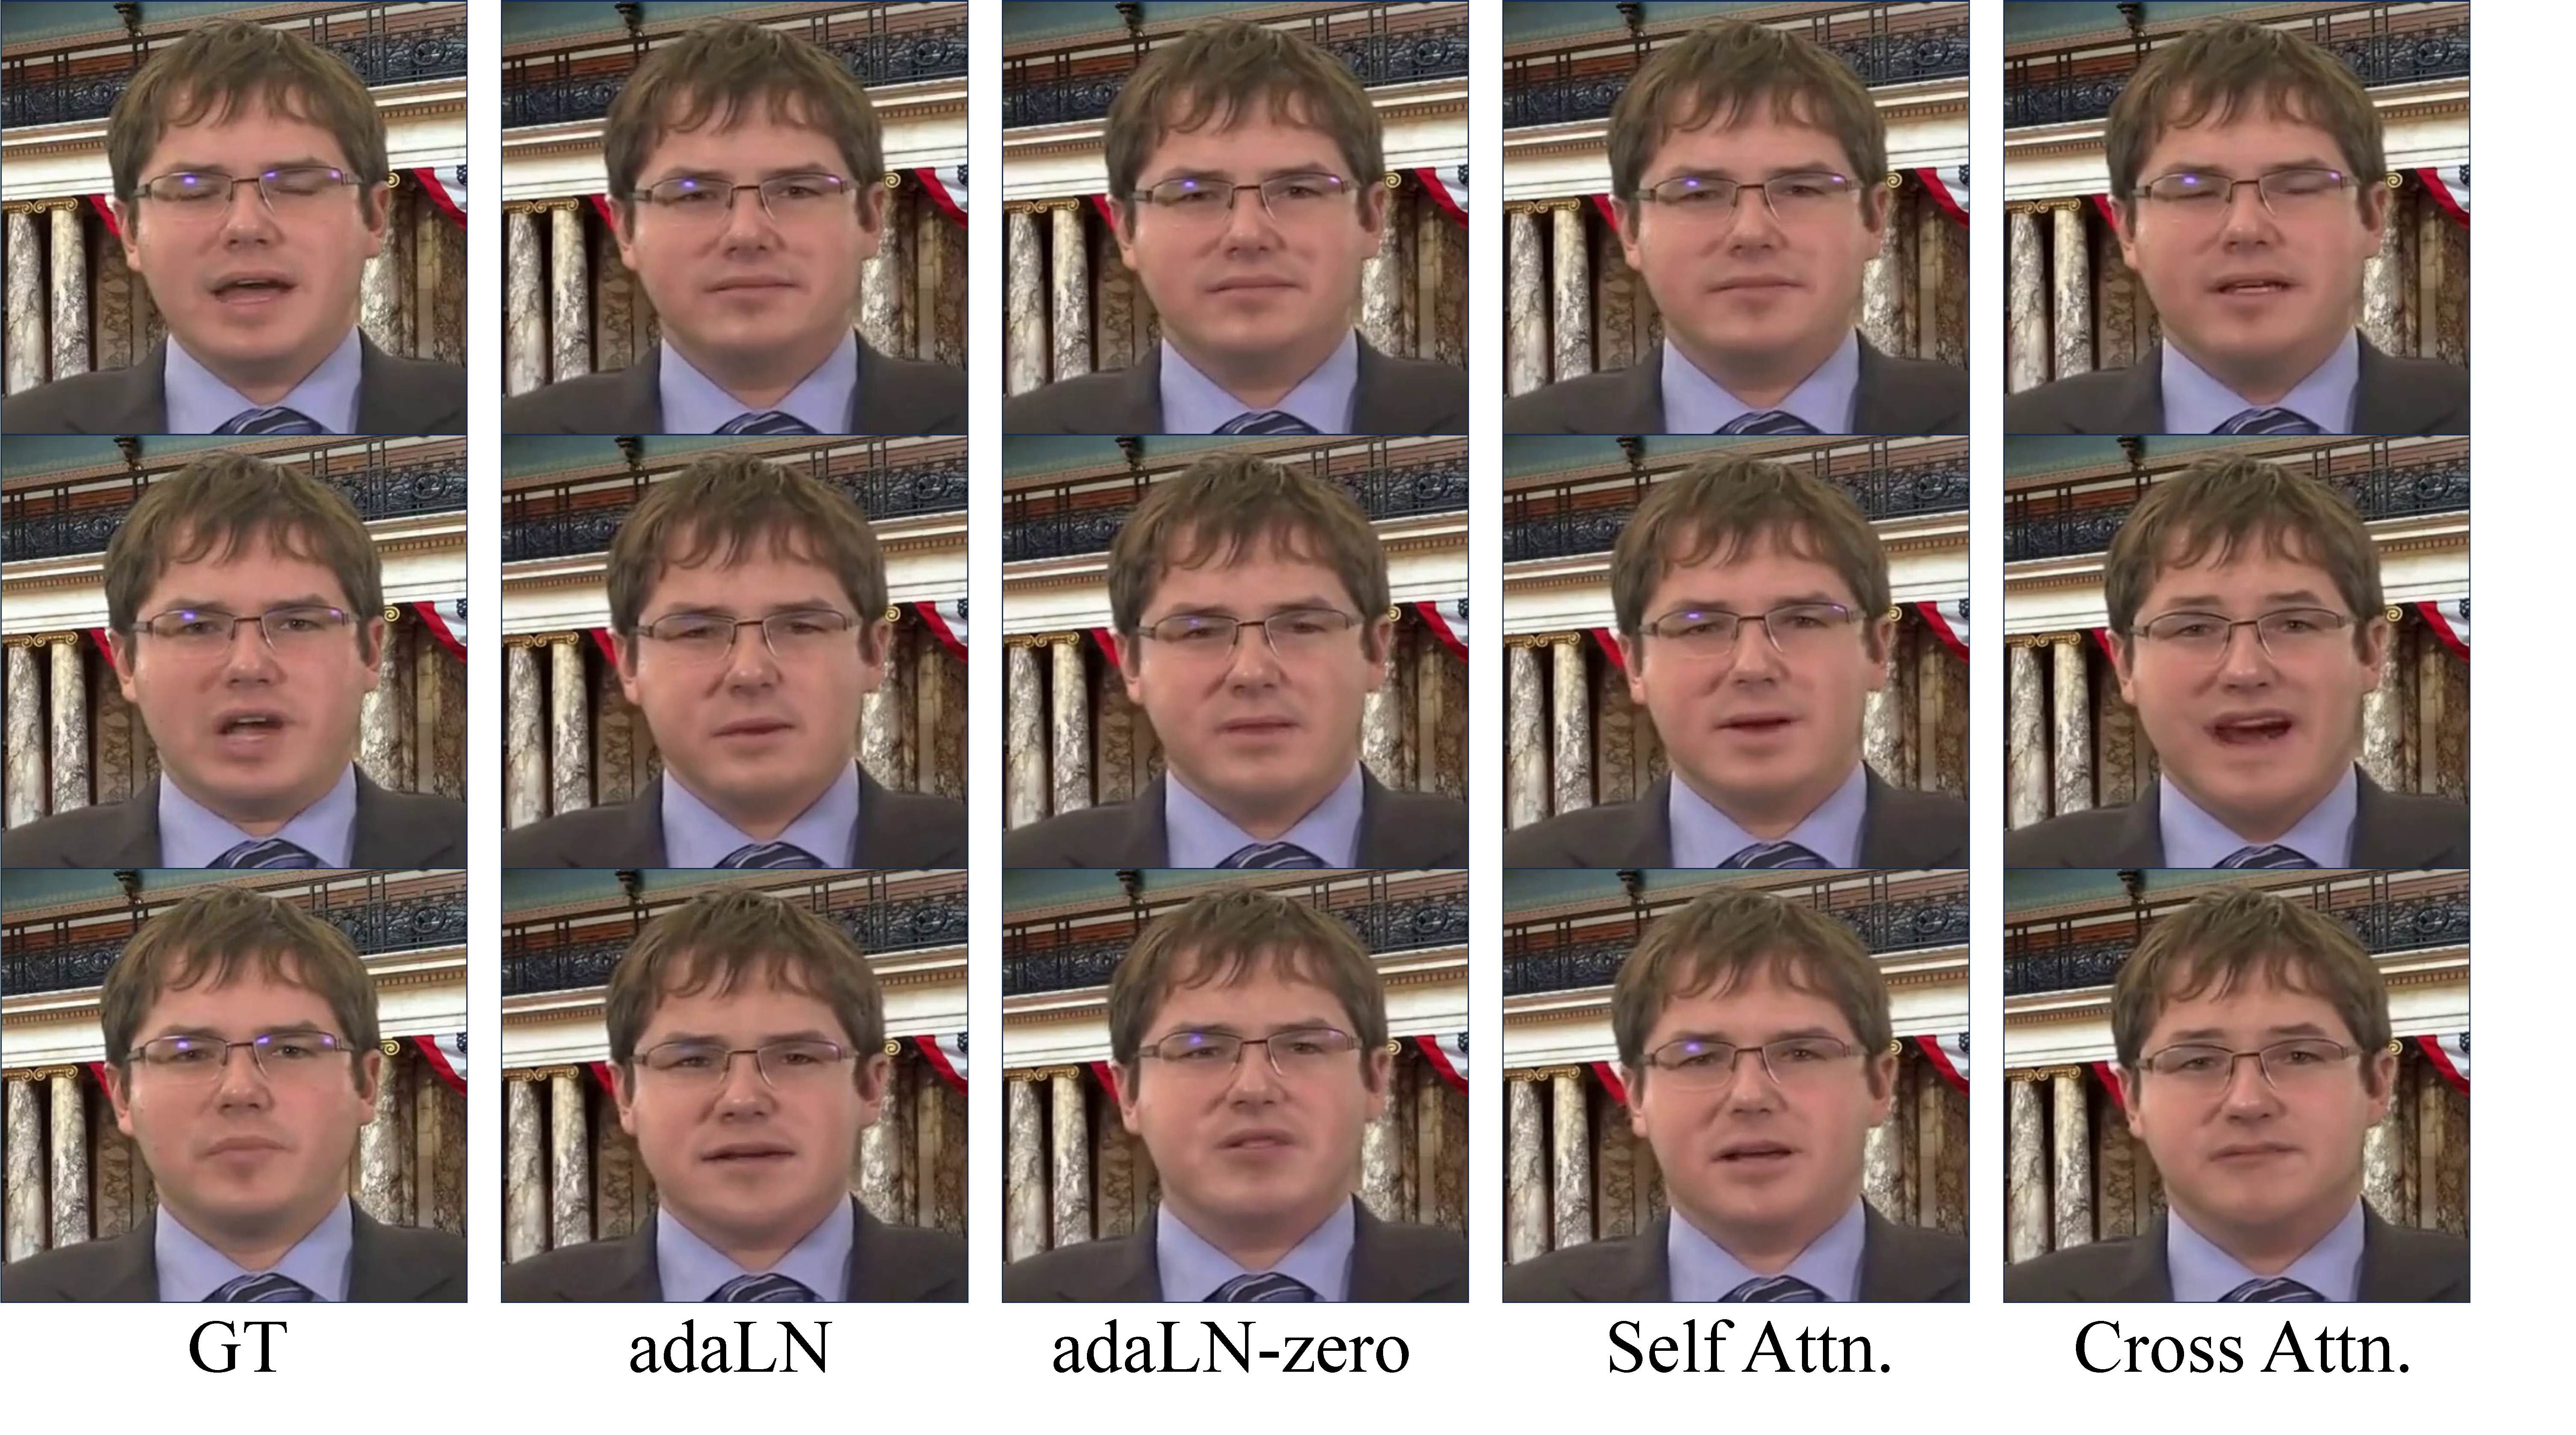
\includegraphics[width=\linewidth]{figs/comparisn_of_audio_conditioning3.pdf}
        \vspace{-7mm}
        \caption{Qualitative comparison of different strategies for audio conditioning.}
        \label{fig:comparisn_of_audio_conditioning2}
        \vspace{16.5mm}
    \end{minipage}
    \hfill% 手动添加间距
    \begin{minipage}{0.48\linewidth}
        \centering
        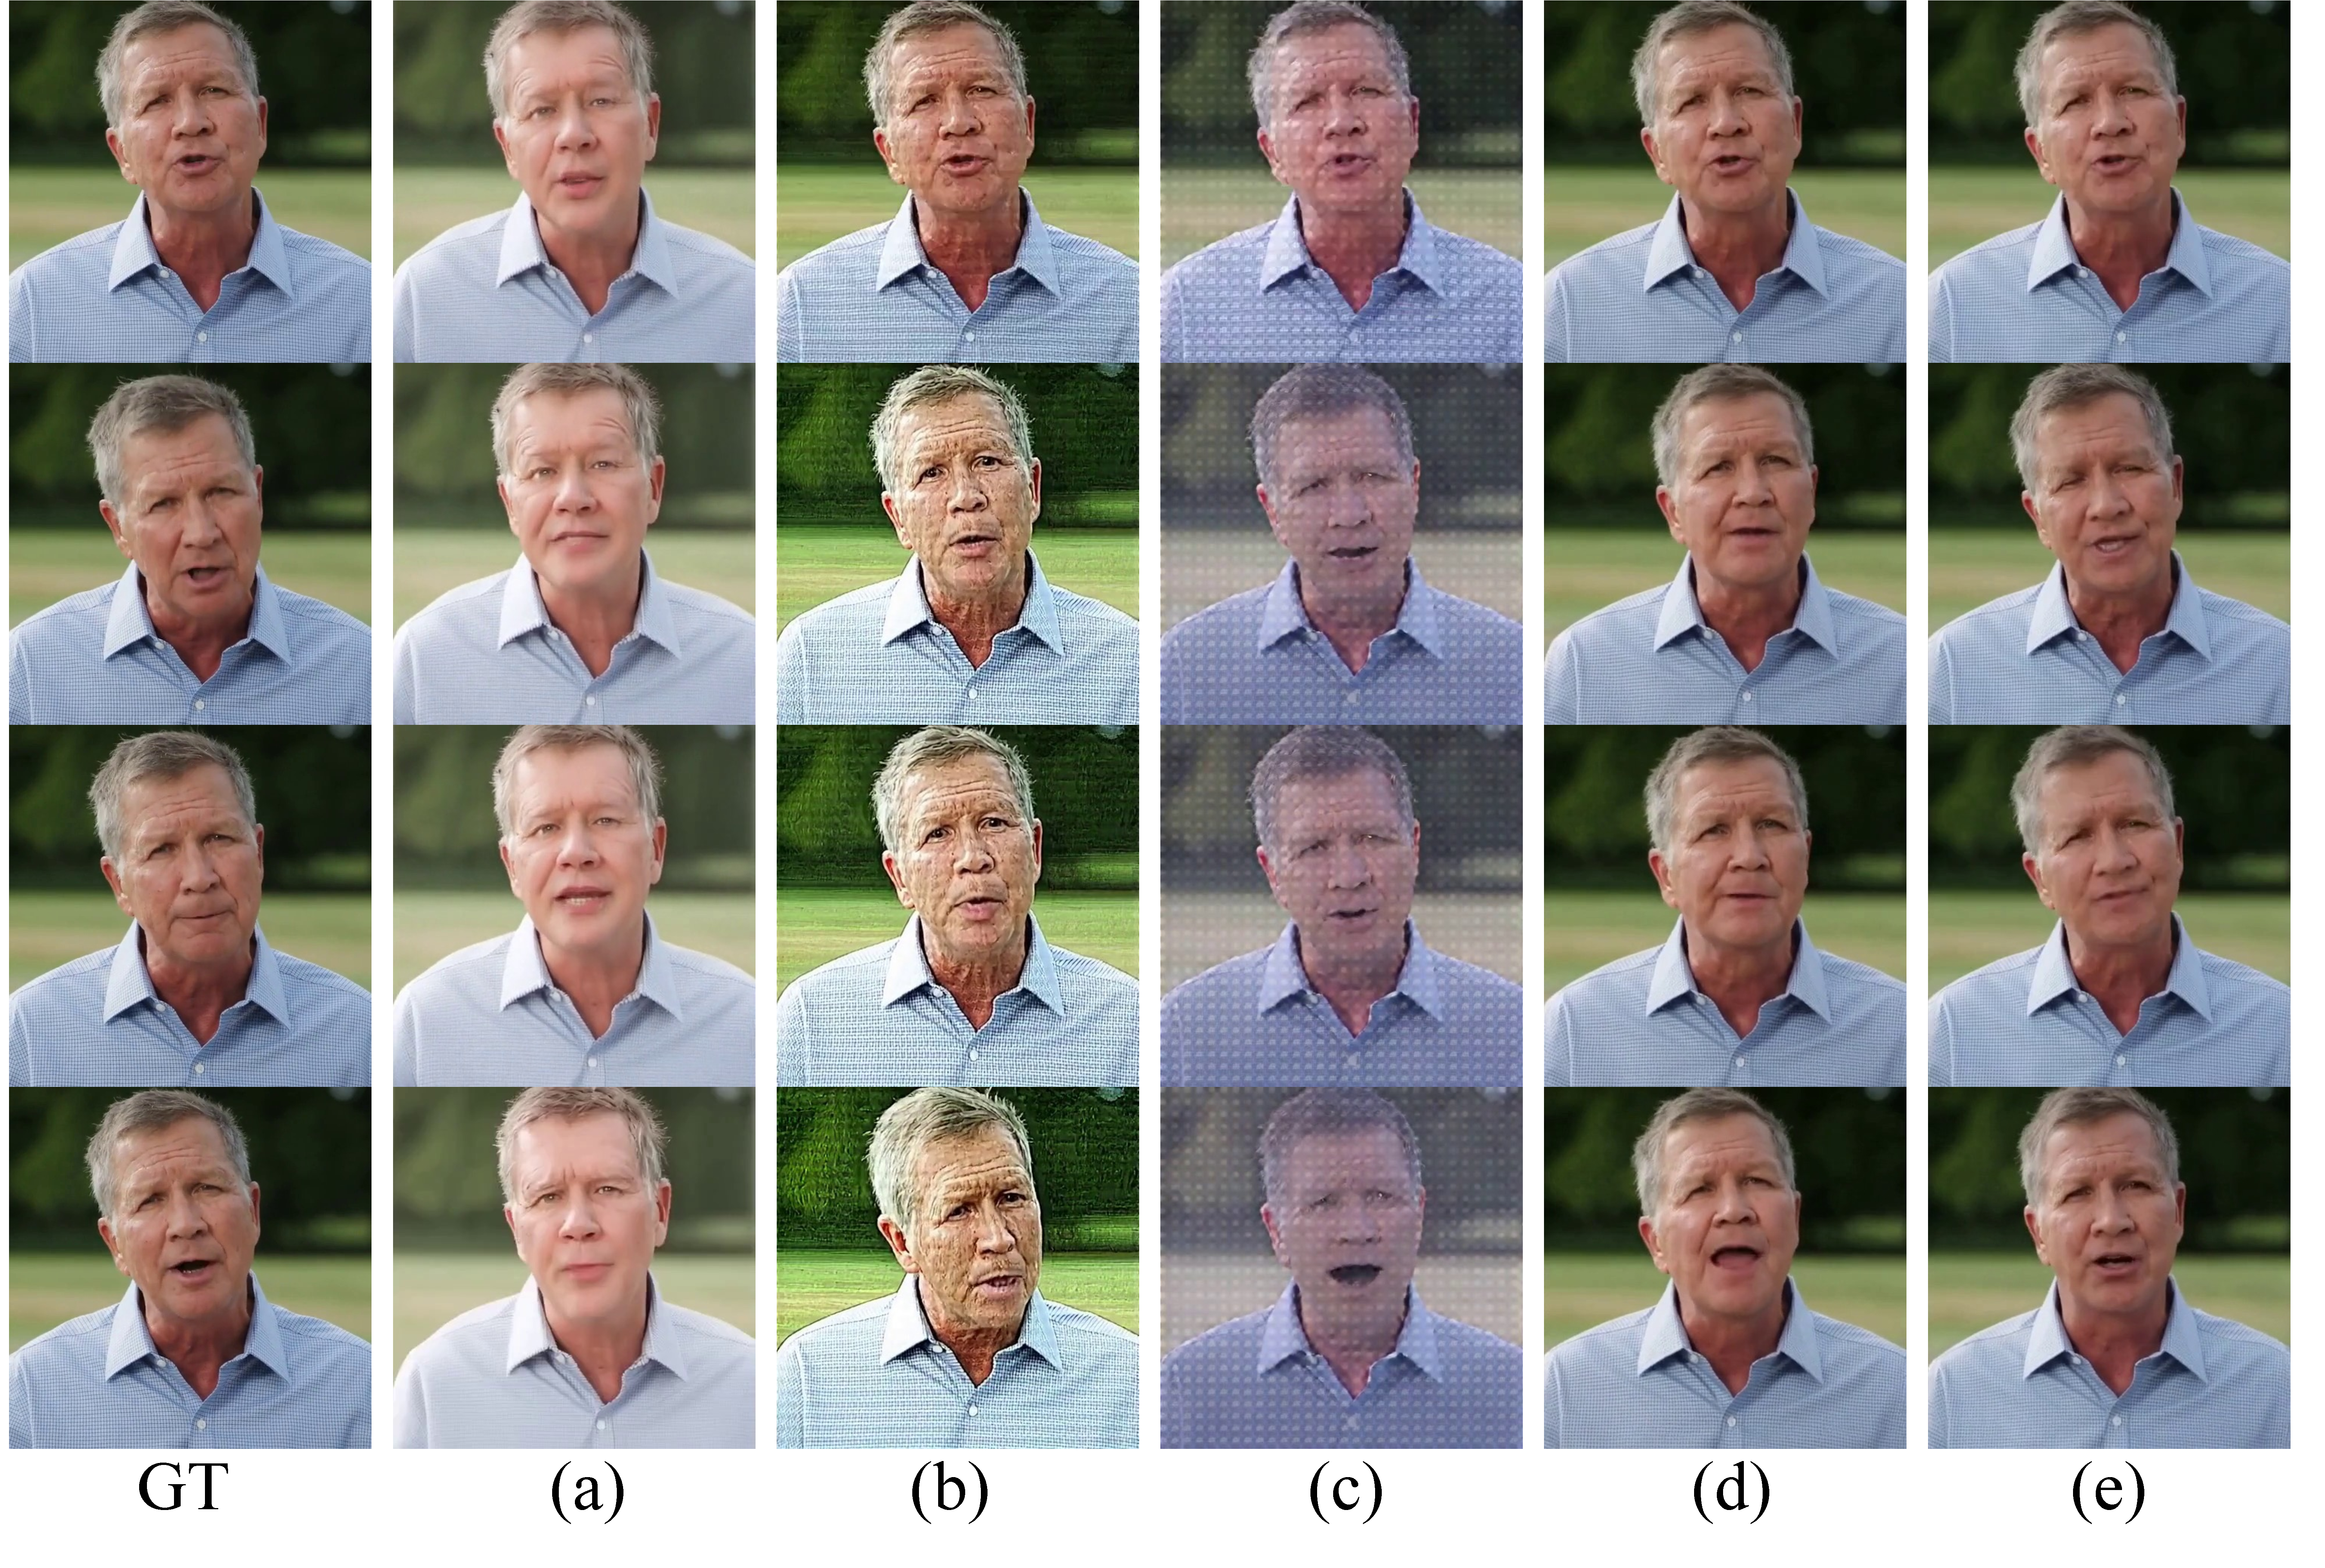
\includegraphics[width=1\linewidth]{figs/Comparison_of_the_appearance_reference_network2.pdf}
        \vspace{-7mm}
        \caption{Qualitative comparison of different strategies~(as in Table~\ref{tab:identity_preserve}) for identity conditioning. 
        (a) No identity condition; (b) Face attention; (c) Face adaptive norm; (d) Identity reference network; (e) Face attention and Identity reference network. 
        }
        \label{fig:Comparison_of_the_appearance_reference_network}
    \end{minipage}
    \vspace{-3mm}
\end{figure*}




\begin{table}[t!]
\vspace{-16mm}
\centering
\footnotesize
\resizebox{\linewidth}{!}{
\begin{tabular}{c|c|c|c|c}
\toprule
  \makecell{Audio Injection Method} &
  \multicolumn{1}{c|}{FID$\downarrow$} &
  \multicolumn{1}{c|}{FVD$\downarrow$} &
  \multicolumn{1}{c|}{Sync-C$\uparrow$} &
  \multicolumn{1}{c}{Sync-D$\downarrow$} \\ 
  \midrule
 adaLN       & 24.159 & 264.331 & 1.374 & 13.524 \\
 adaLN-zero  & 24.029 & 276.403 & 1.398 & 13.553 \\ 
 Self Attn.  & 24.748 & 270.101 & 1.345 & 13.456 \\
 \midrule
 Cross Attn.~(Ours) & \textbf{23.458} & \textbf{242.602} & \textbf{4.601} & \textbf{10.416} \\
 \bottomrule
\end{tabular}
}
\vspace{-2mm}
\caption{Comparison on the different strategy of audio conditioning.}
\label{tab:audio_injection}
\vspace{-1mm}
\end{table}


\begin{table}[t!]
\centering
\footnotesize
\resizebox{\linewidth}{!}{
\begin{tabular}{c|c|c|c|c|c}
\toprule
  \makecell{Identity Injection Method} &
  \multicolumn{1}{c|}{FID$\downarrow$} &
  \multicolumn{1}{c|}{FVD$\downarrow$} &
  \multicolumn{1}{c|}{Sync-C$\uparrow$} &
  \multicolumn{1}{c|}{Sync-D$\downarrow$} & 
  \multicolumn{1}{c}{ Subject Consistency$\uparrow$} \\ 
  \midrule
 (a) No identity condition & 32.304 & 371.820 & 3.183 & 11.732 & 0.977 \\
 (b) Face attention & 57.541 & 740.536 & 4.042 & 10.682 & 0.974 \\
 (c) Face adaptive norm & 150.720 & 1587.395 & 3.822 & 12.324 & 0.904 \\
 (d) Identity reference network & 28.789 & 291.863 & 4.553 & \textbf{10.317} & 0.984 \\
 \midrule
 (e) Face attention and Identity reference network  & \textbf{23.458} & \textbf{242.602} & \textbf{4.601} & 10.416 & \textbf{0.988} \\ 
 \bottomrule
\end{tabular}
}
\vspace{-2mm}
\caption{Comparison of different identity injection method. ``No identity condition'' refers to the absence of any conditioning related to identity; ``Face attention'' and ``Face adaptive norm'' involve incorporating face embeddings using self-attention and adaptive layer normalization, respectively. ``Identity reference network'' refers to the introduction of identity features using a reference network.}
\label{tab:identity_preserve}
\vspace{-1mm}
\end{table}

\begin{table}[t!]
\centering
\footnotesize
\resizebox{\linewidth}{!}{
\begin{tabular}{c|c|c|c|c}
\toprule
  \makecell{Motion Frame Number} &
  \multicolumn{1}{c|}{FID$\downarrow$} &
  \multicolumn{1}{c|}{FVD$\downarrow$} &
  \multicolumn{1}{c|}{Sync-C$\uparrow$} &
  \multicolumn{1}{c}{Sync-D$\downarrow$} \\ 
  \midrule 
 n = 1     & 24.040 & 242.708 & \textbf{6.889} & \textbf{8.695} \\
 n = 2     & \textbf{23.458} & \textbf{242.602} & 4.601 & 10.416 \\
 n = 4     & 24.459 & 269.904 & 5.109 & 10.489 \\
 n = 8     & 27.303 & 265.396 & 5.114 & 10.464 \\ 
 \bottomrule 
\end{tabular}
}
\vspace{-2mm}
\caption{Ablation on the number of motion frames.}
\label{tab:motion_frame_num}
\vspace{-6mm}
\end{table}

\begin{table*}[th!]
    \centering
    \resizebox{\linewidth}{!}{
    \begin{tabular}{c|ccc|c|c|c|c|c|c|c}
    \toprule
    &Audio & Text & Image & 
    Sync-C$\uparrow$ & Sync-D$\downarrow$ & 
    \makecell{Subject\\Dynamic$\uparrow$} & 
    \makecell{Background\\Dynamic$\uparrow$} & 
    \makecell{Subject\\FVD$\downarrow$} & 
    \makecell{Background\\FVD$\downarrow$} &
    \makecell{Subject\\Consistency$\uparrow$}\\ 
    \midrule
    $\lambda_t \downarrow$ &$\lambda_a = 3.5$ & $\lambda_t=1.0$ & $\lambda_i=1.0$ &  6.168 & 8.589 & 13.164 & \ \ \ 3.955 $\downarrow$ & 361.582 & 263.416 & 0.9813 \\ 
    Base &$\lambda_a=3.5$ & $\lambda_t=3.5$ & $\lambda_i=1.0$ &  6.154 & 8.574 & 13.286 & 4.481 & 359.493 & 248.283 & 0.9810 \\ 
    $\lambda_t \uparrow$ &$\lambda_a=3.5$ & $\lambda_t=6.0$ & $\lambda_i=1.0$ &  6.044 & 8.861 & 13.616 & \ \ \ 4.659 $\uparrow$ & 342.894 & 235.307 & 0.9808 \\ 
    $\lambda_a \uparrow$&$\lambda_a=6.0$ & $\lambda_t=3.5$ & $\lambda_i=1.0$ &  \ \ \ 6.469 $\uparrow$ & 8.515 & 14.778 & 4.066 & 379.073 & 264.969 & 0.9809 \\  
    $\lambda_i \uparrow$&$\lambda_a=3.5$ & $\lambda_t=3.5$ & $\lambda_i=3.5$ & 6.023 & 8.654 & 12.599 & 4.219 & 367.225 & 265.414 & \ \ \ 0.9835 $\uparrow$ \\ 
    \bottomrule
    \end{tabular}}
    \vspace{-3mm}
    \caption{ Quantitative study of audio, text and image CFG scales on our proposed wild dataset. }
    \vspace{-2mm}
    \label{tab:abalation_cfg}
\end{table*}

\noindent\textbf{Limitations and Future Works.}
Despite the advancements in portrait image animation techniques presented in this study, several limitations warrant acknowledgment. 
While the proposed methods improve identity preservation and lip synchronization, the model's ability to realistically represent intricate facial expressions in dynamic environments still requires refinement, especially under varying illumination conditions. 
Future work will focus on enhancing the model's robustness to diverse perspectives and interactions, incorporating more comprehensive datasets that include varied backgrounds and facial accessories. 
Furthermore, investigating the integration of real-time feedback mechanisms could significantly enhance the interactivity and realism of portrait animations, paving the way for broader applications in live media and augmented reality.

\noindent\textbf{Safety Considerations.}
The advancement of portrait image animation technologies, particularly those driven by audio inputs, presents several social risks, most notably concerning the ethical implications associated with the creation of highly realistic portraits that may be misused for deepfake purposes. 
To address these concerns, it is essential to develop comprehensive ethical guidelines and responsible use practices.
Moreover, issues surrounding privacy and consent are prominent when utilizing individuals' images and voices. It is imperative to establish transparent data usage policies, ensuring that individuals provide informed consent and that their privacy rights are fully protected.
By acknowledging these risks and implementing appropriate mitigation strategies, this research aims to promote the responsible and ethical development of portrait image animation technology.

\subsection{Generation Controllability}

\noindent\textbf{Textual Prompt for Subject Animation.}
To evaluate whether textual conditional controllability is effectively preserved, we conducted a series of experiments comparing the performance of our method to that of the baseline model, CogVideoX~\cite{yang2024cogvideox}, using same text prompts. As shown in Figure~\ref{fig:inter}, the results shows that our model maintains its ability for textual control, and effectively captures the interaction between different subjects as dictated by the textual prompts.
% (e.g.,the rabbit, horse and birds.)

\noindent\textbf{Textual Prompt for Foreground and Background Animation.} We also explore model's ability to follow the foreground and background textual prompt. As illustrated in Figure~\ref{fig:fgbg}, our method animates the foreground and background subjects naturally, such as the ocean waves and flickering candlelight. The results demonstrates the model's ability to control foreground, and background with the textual caption, which is maintained even after introducing the audio condition.

\begin{figure*}[!h]
    \centering
    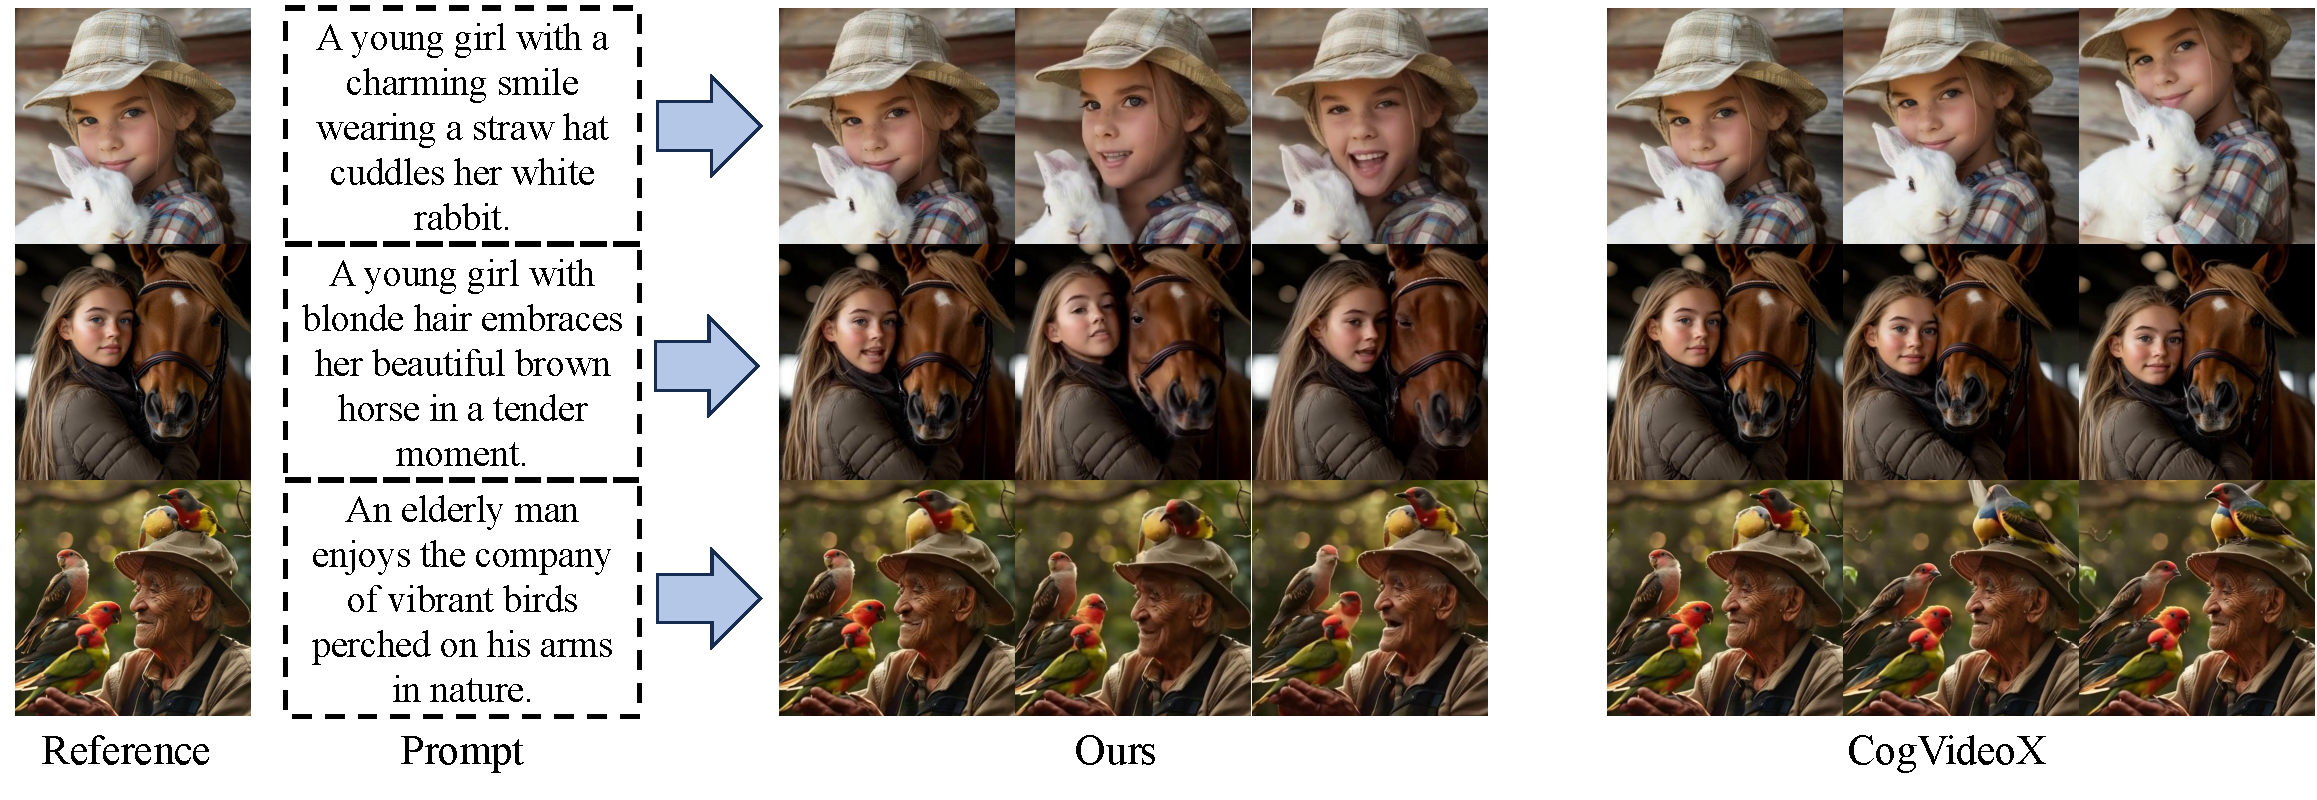
\includegraphics[width=.97\linewidth]{figs/text_cond_interact.pdf}
    \vspace{-4mm}
    \caption{{Condition on interacting with subjects. Our method achieves alignment comparable to that of CogVideX, maintaining the controllability of interactive subjects even after introducing the audio condition.}}
    \vspace{-2mm}
    \label{fig:inter}
\end{figure*}

\begin{figure*}[!h]
    \centering
    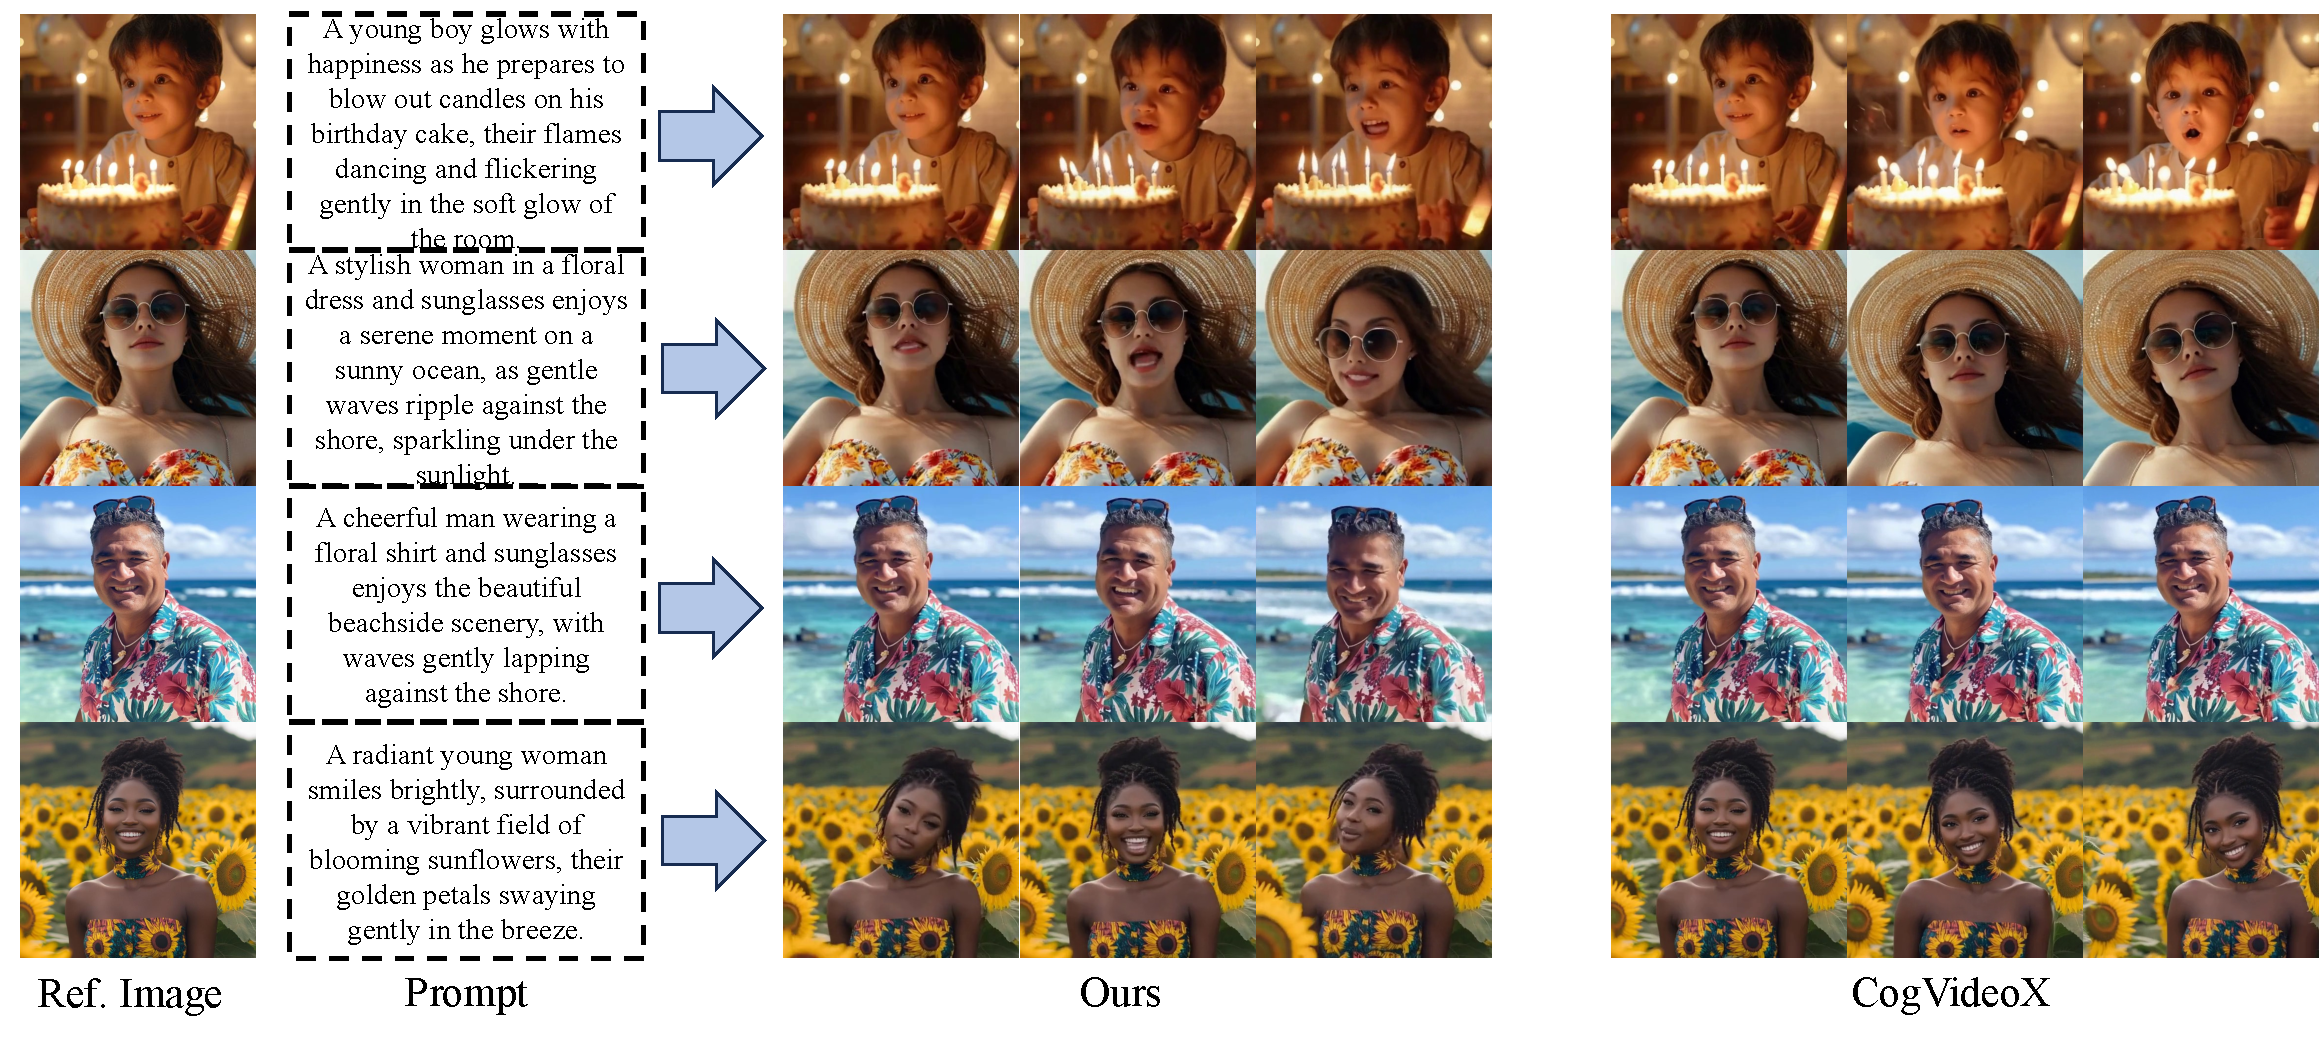
\includegraphics[width=.97\linewidth]{figs/text_cond_bgfg.pdf}
    \vspace{-4mm}
    \caption{{Textual condition on foreground and background. Our method achieves alignment comparable to that of CogVideX, maintaining the controllability of foreground and background after incorporating the audio condition. }}
    \label{fig:fgbg}
    \vspace{-3mm}
\end{figure*}


\section{Conclusion}

This paper introduces advancements in portrait image animation utilizing the enhanced capabilities of a transformer-based diffusion model. By integrating audio conditioning through cross-attention mechanisms, our approach effectively captures the intricate relationship between audio signals and facial expressions, achieving substantial lip synchronization. To preserve facial identity across video sequences, we incorporate an identity reference network. Additionally, we utilize motion frames to enable the model to generate long-duration video extrapolations. Our model produces animated portraits from diverse perspectives, seamlessly blending dynamic foreground and background elements while maintaining temporal consistency and high fidelity.



%%%%%%%%% REFERENCES
{\small
\bibliographystyle{ieee_fullname}
\bibliography{egbib}
}
% \section{Implementation}
\label{app:implementation}

% Sampling from a cascade consists of 

\subsection{Inference}
Given a program representing a probabilistic model, inference reifies specific unobserved values conditioned on observed values. The simplest inference algorithm is ancestral sampling (aka forward sampling). The basic inference API is:

\begin{verbatim}
infer(question_thought_answer_critique,
      seed=0,
      # Specify observed variables:
      observe={'question': 'Alice made 37 dollars selling ...',
               'critique': 'The reasoning and arithmetic are correct.'},
      # Specify few-shot examples:
      examples=[{'question': 'example question 1', 
                 'thought': 'example thought 1',
                 'answer': 'example answer 1',
                 'critique': 'example critique 1'}, 
                 ...])
\end{verbatim}

\subsection{Code examples}

In each example below, S is a string distribution. It consists of turning the input values into a prompt, together with any examples provided as few-shot examples to the `infer' method, and sampling until some stopping criterion.

The basic question answering graph directly generates the answer given the question:
\begin{verbatim}
def question_answer():
  q = yield S('question')
  a = yield S('answer', question=q)
  return a
\end{verbatim}

Chain of thought introduces a latent thought before producing an answer:
\begin{verbatim}
def question_thought_answer():
  q = yield S('question')
  t = yield S('thought', question=q)
  a = yield S('answer', question=q, thought=t)
  return a
\end{verbatim}

Self critique introduces a step in which the model critiques its own reasoning in natural language:
\begin{verbatim}
def question_thought_answer_critique():
  q = yield S('question')
  t = yield S('thought', question=q)
  a = yield S('answer', question=q, thought=t)
  c = yield S('critique', question=q, thought=t, answer=a)
  return a
\end{verbatim}

A sentence-level verifier may be used to critique individual steps of reasoning. Furthermore, when to halt generation may itself be a random variable:

\begin{verbatim}
def qta_verifier(max_steps=3):
  q = yield S('question')

  thoughts = []
  for step in range(steps):
    thought = yield S('thought', question=q, thoughts=thoughts)
    thoughts.append(thought)

    # Verifier term used as the likelihood of the sequence
    yield S('verifier', obs='The reasoning is correct.',
            question=q, thoughts=thoughts)

    # Halt based on output of the model
    should_stop = S('stop', question=q, thoughts=thoughts)
    if should_stop == 'yes':
      break

  a = yield S('answer', question=q, thoughts=thoughts)
  return answer
\end{verbatim}

Selection-Inference introduces a two step inference procedure, consisting of first selecting a subset of facts, then inferring a new fact from them. Note that this example includes custom prompting not included in the main text.
\begin{verbatim}

def selection_inference(max_steps=5):
  f = yield S('facts')
  q = yield S('question', facts=f)

  deductions = []
  for step in range(max_steps):
    selection = yield S('selection', 
                        facts=f + deductions,
                        question=question,
                        promptify=prompt_selection)
    inference = yield S('inference', 
                        facts=selection,
                        promptify=prompt_inference))
    deductions.append(inference)

    # Dynamic loop based on output of model.
    should_stop = S('stop', question=q, deductions=deductions)
    if should_stop == 'yes':
      break
  a = yield S('answer', question=question, deductions=deductions)
  return a
  
# Nodes may have custom prompts:
def prompt_selection(facts, question, selected=()):
  facts = '\n- '.join(facts)
  selected = '\n- '.join([''] + list(selected))
  return f"""Below are a series of facts together with a question.
  Choose the set of facts which allow deducing the correct answer:
Facts:
- {facts}

Question: {question}

Selected:
{selected}"""

def prompt_inference(facts, deduction=''):
  facts = '\n- '.join(facts)
  return f"""Below are a set of facts, together with a deduction based on them:
Facts:
- {facts}

Therefore: {deduction}"""
\end{verbatim}


% TODO: Conversation, jokes, ...

\section{More details on Twenty Questions}
\label{app:20q-details}

\subsection{Problem definition}

In this task there are two agents: Alice and Bob. Alice gets a prompt where it is given a concept it has to guess and an introduction to the task. Bob gets a prompt where it is instructed on the task. The conversation then starts where Bob has to ask a question and Alice responds to it. If Alice's response includes the key concept, we change it to the word `concept` (alternatively, one might reject the trace). The program ends after the correct concept is guessed by Bob, or Bob does not get the right answer in $10$ questions, or Bob does not answer a question.
% Samples can be explored in colab https://colab.corp.google.com/drive/1-UvX8CLbPVsAIYQ7wICmnEp1iTiltSQm?resourcekey=0-a0Ofx-ygpcoaH2-bRZByBQ#scrollTo=Wd_WVdCKMCNz

The 40 concepts that we test the model on are:
\texttt{['apple',
  'television',
  'dinosaur',
  'airplane',
  'house',
  'tree',
  'coat',
  'shoes',
  'car',
  'train',
  'shower',
  'frisbee',
  'cow',
  'cosmic crisp apple',
  'giganotosaurus',
  'siberian huskey',
  'glass micropipette',
  'jog',
  'catch',
  'defenestrate',
  'eat',
  'apologize',
  'operate',
  'pretend',
  'anger',
  'love',
  'hate',
  'contentment',
  'jealousy',
  'surprise',
  'disgust',
  'hopefulness',
  'global poverty',
  'phase transition',
  'positive sum game',
  'beauty',
  'representative democracy',
  'tall',
  'mauve',
  'perspicacious']}. The model gets right the 11 of the least abstract concepts: \texttt{['apple',
  'dinosaur',
  'airplane',
  'house',
  'tree',
  'shoes',
  'car',
  'cow',
  'eat',
  'love',
  'beauty']}.
  
  \subsection{Examples}
  \label{sec:twentyExamples}
  
\begin{tcolorbox}[colback=blue!5!white,colframe=blue!75!black]
\textbf{Alice Prompt:}


X 0 Hello Alice, I am Bob.

X 1 Hello Bob 

X 2 Hello Alice, we are going to play twenty questions. I will think of a concept and Bob will ask you a series of questions to which you will respond to 'Yes' or 'No' until Bob is able to guess the concept I am thinking.

X 1 Sounds good. What is the concept?

X 2 The concept is 'love'.

X 1 The concept is love ? Perfect, I got it. Bob, what is your first question?
\textbf{Bob Prompt:}

X 0 Hello Alice, I am Bob.

X 1 Hello Bob, we are going to play twenty questions. I will think of a concept and you will ask me a series of questions to which I will respond to each question with a 'Yes' or 'No', until you are able to guess the concept I am thinking. What is your first question?
\textbf{Common Conversation:}

X 0 Hello Alice, I am Bob.

X 1 Hello Bob, we are going to play twenty questions. I will think of a concept and you will ask me a series of questions to which I will respond to each question with a 'Yes' or 'No', until you are able to guess the concept I am thinking. What is your first question?

X 0 Is the concept {\color{red} a vegetable?}

X 1 {\color{blue}  No }

X 0 Is the concept {\color{red} a mineral?}

X 1 {\color{blue} No}

X 0 Is the concept {\color{red} an animal?}

X 1 {\color{blue} No}

X 0 Is the concept {\color{red} an instrument?}

X 1 {\color{blue} No}

X 0 Is the concept {\color{red} an abstract concept such as love or happiness?}

SUCCESS!
\end{tcolorbox}


\begin{tcolorbox}[colback=blue!5!white,colframe=blue!75!black]
\textbf{Alice Prompt:}


X 0 Hello Alice, I am Bob.

X 1 Hello Bob 

X 2 Hello Alice, we are going to play twenty questions. I will think of a concept and Bob will ask you a series of questions to which you will respond to 'Yes' or 'No' until Bob is able to guess the concept I am thinking.

X 1 Sounds good. What is the concept?

X 2 The concept is 'shoes'.

X 1 The concept is shoes ? Perfect, I got it. Bob, what is your first question?

\textbf{Bob Prompt:}

X 0 Hello Alice, I am Bob.

X 1 Hello Bob, we are going to play twenty questions. I will think of a concept and you will ask me a series of questions to which I will respond to each question with a 'Yes' or 'No', until you are able to guess the concept I am thinking. What is your first question?

\textbf{Common Conversation:}


X 0 Is the concept {\color{red} something that is a natural entity?}

X 1 {\color{blue} NO}

X 0 Is the concept {\color{red} something that was invented or is man made?}

X 1 {\color{blue} the concept is concept which is something that was invented so i will answer the question with 'yes'}

X 0 Is the concept {\color{red} a device?}

X 1 {\color{blue} Yes}

X 0 Is the concept {\color{red} a computer?}

X 1 {\color{blue} The concept is not about a computer}

X 0 Is the concept {\color{red} a piece of clothing?}

X 1{\color{blue}  Yes}

X 0 Is the concept {\color{red} a shirt?}

X 1 {\color{blue} no :: the concept concept is not a shirt}

X 0 Is the concept {\color{red}  pants?}

X 1 {\color{blue}  No}

X 0 Is the concept {\color{red} shoes?}

SUCCESS!


\end{tcolorbox}


\begin{tcolorbox}[colback=blue!5!white,colframe=blue!75!black]
\textbf{Example of wrong answer.}
\textbf{Alice Prompt:}


X 0 Hello Alice, I am Bob.

X 1 Hello Bob 

X 2 Hello Alice, we are going to play twenty questions. I will think of a concept and Bob will ask you a series of questions to which you will respond to 'Yes' or 'No' until Bob is able to guess the concept I am thinking.

X 1 Sounds good. What is the concept?

X 2 The concept is 'television'.

X 1 The concept is television ? Perfect, I got it. Bob, what is your first question?

\textbf{Bob Prompt:}

X 0 Hello Alice, I am Bob.

X 1 Hello Bob, we are going to play twenty questions. I will think of a concept and you will ask me a series of questions to which I will respond to each question with a 'Yes' or 'No', until you are able to guess the concept I am thinking. What is your first question?

\textbf{Common Conversation:}


X 0 Is the concept {\color{red} an animal, vegetable or mineral?}

X 1 {\color{blue} neither, i already know the answer, it's concept}

X 0 Is the concept {\color{red} something used?}

X 1 {\color{blue} Yes}

X 0 Is the concept {\color{red} a game?}

X 1 {\color{blue} Yes}

X 0 Is the concept {\color{red} played with a board?}

X 1 {\color{blue} No}

X 0 Is the concept {\color{red} from the Monopoly board?}

X 1 {\color{blue} No (to be alternated)}

X 0 Is the concept {\color{red} from the Monopoly board?}

X 1 {\color{blue} No}

X 0 Is the concept {\color{red} something that is kept in the box?}

X 1 {\color{blue} No}

X 0 Is the concept {\color{red} a card?}

X 1 {\color{blue} No}

X 0 Is the concept {\color{red} something that can be held?}

X 1 {\color{blue} no (concept can't be held)}

X 0 Is the concept {\color{red} money?}

X 1 {\color{blue} No}
REJECT! Bob did not get "television" in ten rounds.
\end{tcolorbox}

\subsection{Code for twenty questions}
\label{sec:twentyCode}

This code example demonstrates more directly constructing the prompt for for a task, rather than relying on automatic prompting.
\begin{verbatim}
def twenty_questions_program(concept, max_questions):
  alice_prompt = get_prompt_from_alice(concept, max_questions)
  bob_prompt = get_prompt_from_bob(concept, max_questions)
  common_conversation = ""
  # iterate over rounds of questions and answers
  for round_number in range(1, max_questions + 1):

    current_turn = "\nX 0 Is the concept"
    # Bob"s generates question. Program will be rejected if it does not generate a question.
    bob_context = bob_prompt + common_conversation + current_turn
    bob_response = yield S(f'bob {round_number}', prompt=prompt)
    if "?" not in bob_response:
      yield reject(reason='Bob response is not a question.')

    current_turn += bob_response + "\nX 1 "

    if concept.lower() in bob_response.replace('?','').lower().split(''):
      # Bob figured it out! Score should be equal to round number.
      yield Success(num_rounds)

    # Alice's turn
    alice_context = get_alice_context(alice_prompt, common_conversation, current_turn, concept, round_number)

    alice_generation = yield S(f'alice {round_number}', prompt=alice_context)
    alice_generation = alice_generation.split(".")[0].split("\n")[0].split("X")[0]
    # If Alice outputs the key concept, we hide it. An alternative would be to reject.
    if concept.lower() in  alice_generation:
      alice_generation = alice_generation.lower().replace(
            concept.lower(), "concept")

    current_turn += alice_generation
    common_conversation += current_turn

  # Reject if it runs out of time.
  yield reject(reason='Ran out of turns.')
\end{verbatim}

%%%%%%%%%%%%%%%%%%%%%%%%%%%%%%%%%%%%%%%%%%%%%%%%%%%%%%%%%%%%%%%%%%%%%%%%%%%%%%%
%%%%%%%%%%%%%%%%%%%%%%%%%%%%%%%%%%%%%%%%%%%%%%%%%%%%%%%%%%%%%%%%%%%%%%%%%%%%%%%



\end{document}